%%%%%%%%%%%%%%%%%%%%%%%%%%%%%%%%%%%%%%%%%%%%%%%%%%%%%%
\documentclass[journal]{IEEEtran} 

\usepackage[utf8]{inputenc}
\usepackage{multirow}
\usepackage{booktabs}
\usepackage{siunitx}
\usepackage[colorlinks=true, allcolors=blue]{hyperref}
% \usepackage{amsmath}
\usepackage{amsfonts}
\usepackage{soul} %ONLY FOR THE DRAFT VERSION, REMOVE AFTERWARDS
\usepackage{stfloats}
\usepackage{silence}
\usepackage{multirow}
\usepackage{algorithmic}
\usepackage{fancyhdr,graphicx,amsmath,amssymb}
% \usepackage[ruled,vlined]{algorithm2e}
% \include{pythonlisting}
\usepackage{pifont}
\usepackage{afterpage}
\usepackage{subcaption}
\usepackage{subfloat}
\usepackage{float}
\restylefloat{table}
\usepackage{enumitem}
\usepackage{bbding}
\usepackage{todonotes}
\usepackage{caption}
% \captionsetup{belowskip=-5pt} 
\usepackage{makecell}
\usepackage{color,colortbl}
\usepackage{orcidlink}

\usepackage{tikz,xcolor}
\definecolor{lime}{HTML}{A6CE39}
\DeclareRobustCommand{\orcidicon}
{
    
\begin{tikzpicture}
    \draw[lime, fill=lime] (0,0) circle [radius=0.16] 
    node[white] {{\fontfamily{qag}\selectfont \tiny ID}};    \draw[white, fill=white] (-0.0625,0.095) circle [radius=0.007];    
    \end{tikzpicture}
    \hspace{0mm}}
\foreach \x in {A, ..., Z}{%
    \expandafter\xdef\csname orcid\x\endcsname{\noexpand\href{https://orcid.org/\csname orcidauthor\x\endcsname}{\noexpand\orcidicon}}
}
\newcommand{\orcidauthorA}{0000-0003-2020-8186}
\newcommand{\orcidauthorB}{0000-0002-2792-5965}
\newcommand{\orcidauthorC}{0009-0000-4502-8574}
\newcommand{\orcidauthorD}{0000-0001-9480-0356}


% \floatsep %vspace between two adjacent floats
% \intextsep: space left on top and bottom of an in-text float
% \setlength{\textfloatsep}{6pt} % space between last top [t] float or first bottom [b] float and the text in a page
% \setlength{\intextsep}{6pt} % default is 8pt before table/figure for [h]
% \setlength{\dbltextfloatsep}{6pt} % space after two column 
% \setlength{\dblfloatsep}{10pt} %vspace between two adjacent two-column-float
% space above and below equations
% \setlist[enumerate]{itemsep = 0pt, parsep = 0pt, topsep = 0pt} % enumerate spacing setting
% \setlist[itemize]{itemsep = 0pt, parsep = 0pt, topsep = 0pt} % itemize spacing setting
% Decrease space above and below equations
% \setlength{\abovedisplayskip}{3pt}
% \setlength{\belowdisplayskip}{3pt}


% \povidecommand{\lan}[1]{\textcolor{blue}{lan: {#1}}}

\begin{document}

\title{
RoGaussianOCC: An Accurate and Robust Gaussian Occupancy Prediction in\\ Autonomous Driving
}

\author{Gongjin Lan\hspace{-1mm} \Envelope\orcidA{}\hspace{-1mm}, \IEEEmembership{Senior Member, IEEE}, Jianfa Ma, Ziyue Zhao, Qining Qi, Yechong Liu and Qi Hao\hspace{-1mm} \orcidB{}\hspace{-1mm}
% , \IEEEmembership{Senior Member, IEEE} 
\thanks{This work was supported in part by the National Natural Science Foundation of China (62261160654), the Shenzhen Fundamental Research Program (JCYJ20220818103006012, KJZD20231023092600001).
% the Guangdong Basic and Applied Basic Research Foundation (2021A1515110641). 
% (Gongjin Lan and Zexuan Jia contributed equally to this work; 
Corresponding author: Gongjin Lan (e-mail: langj@sustech.edu.cn).
}
\thanks{
Gongjin Lan, Jianfa Ma, Ziyue Zhao, Qining Qi, Yechong Liu, and Qi Hao are with the Department of Computer Science and Engineering, Southern University of Science and Technology, Shenzhen, 518055, China.}
% \thanks{Qi Hao is with the Department of Computer Science and Engineering, Southern University of Science and Technology, China.}
% \vspace{-9pt}
}

% The paper headers
\markboth{Journal of \LaTeX\ Class Files,~Vol.
% ~14, No.~8, August~2015
}%
{Shell \MakeLowercase{\textit{et al.}}: Bare Demo of IEEEtran.cls for IEEE Journals}


% make the title area
\maketitle

% As a general rule, do not put math, special symbols or citations
% in the abstract or keywords.
\begin{abstract}
In autonomous driving, occupancy prediction is an emerging and mainstream perception method that predicts the spatial occupancy and semantics of 3D voxel grids around the autonomous vehicle from image inputs, providing high robustness in perception, particularly in adverse driving scenes.
However, occupancy prediction generally requires dense occupancy representations with redundant computing.
Recently, Gaussian-based occupancy prediction has shown state-of-the-art performance in autonomous driving. 
However, the existing Gaussian occupancy predictions remain inefficient and non-robust (e.g., occlusion scenarios), with several issues including inefficient Gaussian representation, distortion of the Gaussian distribution, and sparse supervision signals.
In this work, we propose a novel Gaussian occupancy prediction, called RoGaussianOCC, to solve these issues and improve efficiency and robustness by considering the three key novel modules: 1) Gaussian fusion, 2) Gaussian feature aggregation, and 3) perspective supervision.
We conducted an ablation study and compared RoGaussianOCC with state-of-the-art occupancy predictions on the well-known nuScenes dataset.
The results show that the proposed three novel modules contribute to the improvement of occupancy prediction in terms of accuracy and robustness, and our RoGaussianOCC outperforms the existing occupancy predictions (e.g., GaussianFormer).
Finally, we release the open-source code, video description, and datasets to facilitate the development of Gaussian occupancy prediction in autonomous driving.
\end{abstract}

% \noindent
% \textbf{Note to Practitioners:}

% This paper was motivated by the issues of the existing Gaussian occupancy predictions in autonomous driving.
% The existing Gaussian occupancy predictions have many issues, such as inefficient Gaussian representation, Gaussian distribution distortion, and sparse supervision signals.
% This paper suggests a novel Gaussian occupancy prediction, called RoGaussianOCC, to solve these issues by considering spatiotemporal fusion, which consists of three modules: 1) historical Gaussian fusion, 2) Gaussian feature aggregation, and 3) perspective supervision.
% The experiments suggest that the spatio-temporal fusion contributes to the improvement of occupancy prediction, and our RoGaussianOCC outperforms the existing occupancy predictions.
% Our RoGaussianOCC contributes to facilitating the occupancy prediction of autonomous driving.
% In the future, we will apply the proposed RoGaussianOCC to improve the performance of end-to-end autonomous driving models.

% Note that keywords are not normally used for peerreview papers.
\begin{IEEEkeywords}
Autonomous driving, Occupancy prediction, Gaussian splitting, Gaussian fusion.
\end{IEEEkeywords}

% For peer review papers, you can put extra information on the cover
% page as needed:
% \ifCLASSOPTIONpeerreview
% \begin{center} \bfseries EDICS Category: 3-BBND \end{center}
% \fi
%
% For peer-review papers, this IEEEtran command inserts a page break and
% creates the second title. It will be ignored for other modes.

%%%%%%%%%%%%%%%%%%%%%%%%%%%%%%%%%%%%
\section{Introduction}
\label{sec:intro}
%%%%%%%%%%%%%%%%%%%%%%%%%%%%%%%%%%%%

% why this work is important? 
Autonomous driving generally refers to the technology system that controls the vehicle to reach the destination by recognizing the external environment without driver intervention \cite{lan2024sustechgan}.
Current autonomous driving systems significantly benefit from data-driven deep neural networks for powering critical functions such as perception, decision-making, and planning.
Perception is the foundational component of current autonomous driving systems (including end-to-end methods) to understand driving scenes, on which path planning and decision-making rely entirely on the accuracy and reliability of real-time environmental understanding.
Bird’s-eye view (BEV) perception is the mainstream perception pattern, offering advantages in spatial understanding, sensor fusion, decision-making, and system robustness due to its absolute scale and lack of occlusion in describing environments \cite{li2023delving}.
% However, BEV perception provides 2D scene representations and cannot represent 3D scenes.
Particularly, the general BEV-based perception methods often lack robustness in adverse driving scenes typically including the scenes of 1) sudden illumination changes (e.g., oncoming headlight glare, low-angle sun glare, black and white hole effect of tunnel portals), 2) adverse weather conditions (e.g., heavy rain, dense fog, heavy snow, and
dust storm), as shown in \autoref{fig:scenes}.
Fundamentally, the perception challenges of adverse driving scenes are rooted in the limitations of sensor dynamic range and the constraints of data generalization boundaries, commonly referred to as out-of-distribution (OOD) issues. 
Consequently, the general BEV-based methods struggle to correctly identify traffic objects in these typically adverse driving scenes, thereby resulting in traffic accidents involving autonomous vehicles.

\begin{figure}[!ht] \centering
    \includegraphics[width=0.98\linewidth,page=13,trim={61 208 329 93},clip]{figures/figures.pdf}
    \caption{The adverse scenes of autonomous driving, including the scenes of 1) sudden illumination changes (e.g., oncoming headlight glare, low-angle sun glare, black hole effect (at the entrance), and white hole effect of tunnel portals), 2) adverse weather scenes (e.g., heavy rain, dense fog, heavy snow, and dust storm). (Source: Public datasets and the internet)}
    \label{fig:scenes}
\end{figure}

Recently, occupancy perception has emerged as a mainstream perception system for autonomous driving, which observes and understands the spatial 3D occupancy and semantics of 3D voxel grids surrounding the autonomous vehicle from visual inputs, where each voxel is classified as occupied or free \cite{xu2025survey,zhang2024vision}.
Occupancy prediction can represent arbitrarily shaped traffic objects (such as a fallen tree or a leaking truck) that don't fit into standard 3D bounding boxes.
It provides the most critical geometric collision risk information, ensuring the vehicle avoids physical collisions and provides high robustness perception, particularly in adverse driving scenes, which are viewed as the next evolution beyond 3D object detection.
However, the existing occupancy perception methods generally have several issues, including dense scene representations and redundant computation. 


Recently, 3D Gaussians have been applied to occupancy prediction to solve these issues, demonstrating state-of-the-art performance in autonomous driving \cite{huang2024gaussianformer,zuo2024gaussianworld,sun2024gsrender,zhou2025occgs}.
% how is the current state?
% Several studies have investigated Gaussian occupancy predictions in autonomous driving \cite{huang2024gaussianformer,zuo2024gaussianworld,sun2024gsrender,zhou2025occgs}.
% there is a lack of studies that investigate this task under adverse conditions. 
In our preliminary experiments, we observed the performance of the well-known Gaussian occupancy predictions (e.g., GaussianFormer \cite{huang2024gaussianformer}) and analyzed the key issues in these methods. 
Our preliminary experimental results show that existing Gaussian occupancy prediction remains inefficient and non-robust (e.g., occlusion scenarios) with several issues, including 1) inefficient Gaussian representation, 2) Gaussian distribution distortion, and 3) sparse supervision.
In this work, we investigate the three key issues in the current Gaussian occupancy prediction for autonomous driving.
\begin{enumerate} [noitemsep,leftmargin=*,topsep=0pt]
    % 1.基于局部感知的稀疏占用算法的方法，受稀疏卷积和关键点生成的影响，对体素空间位置的尺度局限于特定的区域内。这会导致随机初始化在在空区域的高斯，受限于空间更新的尺度，即使在调整过后仍然拟合了不重要的区域，高斯表示利用率低。
    \item Inefficient Gaussian representation. The scale of the voxel spatial position in local-aware sparse occupancy prediction is limited to a specific area.
    Specifically, the spatial updating scale limits the initialized Gaussians in empty regions.
    % Even after adjustment, it still fits unimportant areas, and the Gaussian representation has low utilization.
    % 2.现有3D高斯占用预测模型主要通过当前帧采样更新高斯参数，难以补全被遮挡区域的高斯分布。且在部分物体被遮挡的情况下，模型无法获取完整的3D结构信息，导致遮挡后视角区域的预测失效。
    \item Gaussian distribution distortion. The existing Gaussian occupancy prediction primarily updates the Gaussian parameters using the current frame, which is insufficient for accurately predicting the Gaussian distribution of occluded areas and the 3D structure of partially occluded objects.
    % In addition, when some objects are occluded, the model cannot obtain complete 3D structural information, resulting in the failure of the prediction of the viewing area after occlusion.
    % 3.当前的3D高斯占用模型，受到对图像特征的稀疏采样的影响，仅有少数受关注区域受到监督，其对backbone的监督信号同样稀疏，导致缺乏早期收敛能力以及跳出局部最优的能力。
    \item Sparse supervision. The current Gaussian occupancy prediction samples image features sparsely, with only a few areas of interest being supervised, resulting in a sparse supervision signal for the training backbone.
\end{enumerate}

\begin{figure*}[!ht] \centering
\includegraphics[width=0.98\textwidth,page=2,trim={180 122 180 100},clip]{figures/figures.pdf}
\caption{The framework of our Gaussian occupancy prediction, RoGaussianOCC, contains three main parts: 1) historical Gaussian fusion, 2) Gaussian feature aggregation, and 3) perspective supervision.}
\label{fig:framework}
\end{figure*}

In this work, we propose a novel Gaussian occupancy prediction method, called RoGaussianOCC, to solve three key issues that improve efficiency and robustness by considering three key modules: 1) historical Gaussian fusion, 2) Gaussian feature aggregation, and 3) perspective supervision, as shown in \autoref{fig:framework}.
To validate the performance, we conduct an ablation study and compare RoGaussianOCC to state-of-the-art occupancy predictions on the well-known nuScenes dataset.
The results show that our RoGaussianOCC outperforms existing well-known occupancy predictions, demonstrating that the proposed three novel modules in our RoGaussianOCC contribute to higher accuracy and robustness in occupancy predictions.
Finally, the open source code, video description, and datasets are available on the page 
% \footnote{\url{to be released}}
\footnote{\url{https://github.com/Pluviophil3/RoGaussianOCC}} 
to facilitate Gaussian occupancy prediction in autonomous driving.
The main contributions of this work can be summarized as:
\begin{enumerate} [noitemsep,leftmargin=*,topsep=0pt]
    \item A historical Gaussian fusion that merges current Gaussian features with historical Gaussian spatial distribution, introducing prior Gaussian features to update the spatial updating scale and reduce inefficient Gaussians in empty regions, thereby improving Gaussian representation efficiency. 
    % 2.现有3D高斯占用预测模型主要通过当前帧采样更新高斯参数，难以补全被遮挡区域的高斯分布。且在部分物体被遮挡的情况下，模型无法获取完整的3D结构信息，导致遮挡后视角区域的预测失效。
    % 2.为了在高维空间隐式融合时序信息，解决遮挡问题，我们提出了Gaussian aggegation模块。该模块在deformable attention阶段通过对连续图像输入的4D时空采样，并聚合高斯query序列，旨在增强 OCC 预测的时序一致性，从而有效缓解高斯在长时间遮挡场景下的分布失真问题。
    \item A Gaussian feature aggregation to alleviate the Gaussian distribution distortion in occlusion scenarios by fusing temporal information, which introduces a 4D spatiotemporal sampling of continuous image inputs and aggregates Gaussian query sequences to improve occupancy prediction in occlusion scenarios.
    % This module samples the 4D space-time of continuous image inputs in the deformable attention stage and aggregates the Gaussian query sequence to enhance the temporal consistency of OCC prediction, thereby effectively alleviating the Gaussian distribution distortion in occlusion scenarios.
    % 3.当前的3D高斯占用模型，受到对图像特征的稀疏采样的影响，仅有少数受关注区域受到监督，其对backbone的监督信号同样稀疏，导致缺乏早期收敛能力以及跳出局部最优的能力.
    % 3.我们采用透视监督作为额外监督信号，旨在使用辅助透视损失函数直接监督image backbone，提升关注区域的在训练中的监督密度，提高占用预测精度的同时，加速了模型的收敛过程。
    \item A novel perspective supervision as an auxiliary loss to improve the supervision density of the areas of interest during training, thus improving occupancy prediction accuracy.
\end{enumerate}


The rest of this paper is organized as follows. 
In \autoref{sec:related}, we review the related work of occupancy prediction in autonomous driving. 
Our method is presented in \autoref{sec:methodology}, including historical Gaussian fusion, Gaussian feature aggregation, and perspective supervision. 
\autoref{sec:experiments} addresses the datasets, evaluation, and experimental setup. 
The results are presented in \autoref{sec:results}. 
Finally, we provide an in-depth discussion in \autoref{sec:discussion} and a conclusion in \autoref{sec:conclusions}.


%%%%%%%%%%%%%%%%%%%%%%%%%%%%%%%%%%%%
\section{Related Work}
\label{sec:related}
We review the related studies from 1) the state-of-the-art occupancy prediction and 2) the Gaussian occupancy prediction in autonomous driving.

\noindent
\textbf{Occupancy Prediction} Many studies have investigated occupancy prediction for autonomous driving.
% Current 3D occupancy prediction mainly contains three branches: 1) image-based methods, 2) LiDAR-based methods, and 3) multi-modal methods. 
Early, Tesla announced the camera-only occupancy network to understand the 3D environment 
% surrounding a vehicle 
according to surround-view RGB images for autonomous driving.
Image-based occupancy predictions are favored for practical deployment due to their low computational and hardware costs \cite{zhang2024vision}.
Many remarkable occupancy networks were proposed to perceive 3D scenes, such as SurroundOcc \cite{wei2023surroundocc}, Occ3D \cite{tian2023occ3d}, OccFormer \cite{zhang2023occformer}, SparseOcc \cite{tang2024sparseocc}.
Specifically, SurroundOcc \cite{wei2023surroundocc} constructs image features at various levels and utilizes 2D-3D attention to elevate low-resolution, high-level semantic features to a coarse-grained 3D voxel space.
Occ3D \cite{tian2023occ3d} proposed an incremental token selection strategy to selectively choose foreground and uncertain voxel tokens during cross-attention computation for adaptive and efficient computation without sacrificing accuracy.
OccFormer \cite{zhang2023occformer} proposed a dual-path Transformer to encode 3D voxels in different directions and utilize a mask classification model for occupancy prediction.
SparseOcc \cite{tang2024sparseocc} introduced a sparse voxel decoder to reconstruct the scene with the sparse geometric structure by modeling only the non-empty regions, significantly reducing the computing.
Although these methods perform remarkably well in occupancy prediction, they employ dense voxels as scene representations, which overlook the occupancy sparsity of natural driving scenes and thus result in a significant amount of redundant computing.

\noindent
\textbf{Gaussian Occupancy Prediction}
Recently, 3D Gaussians have been applied to occupancy prediction to improve occupancy representation efficiency and reduce redundant computing.
GaussianFormer \cite{huang2024gaussianformer} proposed the 3D Gaussians as an efficient object-centric representation for driving scenes.
% Specifically, an object-centric representation describes 3D scenes with sparse Gaussians representing a flexible region of interest and its semantic features. 
Furthermore, an efficient Gaussian-to-voxel splatting generates 3D occupancy predictions by aggregating the neighboring Gaussians.
However, GaussianFormer does not consider the continuity of driving scenarios and ignores the prior information from historical frames.
GaussianFormer-2 \cite{huang2025gaussianformer} proposed a probabilistic Gaussian superposition model, which interprets each Gaussian as a probability distribution of its neighborhood being occupied and conforms to probabilistic multiplication to derive the overall geometry.
% 这个工作在gsformer上进行了改进，优化了计算效率，但仍然局限于单帧推理。
Although GaussianFormer-2 optimized the computational efficiency of GaussianFormer, it remains limited to single-frame occupancy prediction.
GaussianWorld \cite{zuo2024gaussianworld,feng2025gaussian} proposed a Gaussian world model to exploit these priors and infer scene evolution in 3D Gaussian space, which reformulates 3D occupancy prediction as a 4D occupancy forecasting problem conditioned on the current sensor input.
% 因此，基于object-centric 3D semantic Gaussians的OCC方法\cite{gaussianformer}被提出，通过高斯椭球的几何性质刻画场景对象来表示3D空间的场景特征，再将高斯Spatting转化为Occupancy，实现对环境的占用预测。与传统的像素或体素表示不同，object-centric的3D高斯拥有极其灵活的几何性质，能够以可变形的方式适应不同的目标和区域，从而提高计算效率。
% 在 3D 语义高斯 OCC 方向上，已有多个研究探索了其在自动驾驶场景中的应用，主要包括 GaussianFormer 和 GaussianWorld\cite{gaussianworld} 等代表性工作。
% GaussianFormer 采用Cross-Attention，从多尺度图像特征中聚合信息，并迭代调整 3D 高斯的属性，使得高斯拟合 3D 空间分布。这一工作表明，在不牺牲预测精度的前提下，3D 高斯特征可以显著降低计算开销。然而，该方法主要依赖于单帧图像数据进行 OCC 预测，缺乏对连续驾驶场景中的时序信息建模，因此在动态场景中的表现存在一定局限性。
% 针对 GaussianFormer 在时序建模方面的不足，GaussianWorld 提出了一种新的方法，该方法通过构建高斯世界模型来建模驾驶过程中的时序演变，并引入先验知识以优化 OCC 预测。
GSRender \cite{sun2024gsrender} employs 3D Gaussian splatting to simplify the sampling process for occupancy prediction.
EmbodiedOcc \cite{wu2025embodiedocc,wang2025embodiedocc++} is a Gaussian-based framework that formulates an embodied 3D occupancy prediction task to target this practical scenario, which initializes the global scene with uniform 3D semantic Gaussians and progressively updates local regions observed by the embodied agent.
GS-Occ3D \cite{ye2025gs} optimizes an explicit occupancy representation using an Octree-based Gaussian Surfel formulation for ensuring efficiency and scalability.
OccGS \cite{zhou2025occgs} developed a cumulative Gaussian-to-3D voxel splatting method for occupancy prediction using semantic and geometric-aware Gaussian splatting.
VoxelSplat \cite{zhu2025voxelsplat} leverages enhanced semantics supervision through 2D projection and scene flow learning to improve the accuracy of both semantic occupancy and scene flow estimation.
Although these studies have investigated the Gaussian occupancy prediction, the existing Gaussian occupancy predictions remain inefficient and non-robust with several issues including inefficient Gaussian representation, distortion of the Gaussian distribution, and sparse supervision signal.
Specifically, they have not considered the global temporal modeling for driving scenes, particularly occlusion scenes.


% 但该方法仅依据历史信息进行高斯对齐，并预测动态物体的运动轨迹，未能实现对整个场景的全局时间建模，在长时间遮挡的情况下容易出现信息丢失的问题。
% In this paper, we propose a temporal fusion method by combining the historical Gaussian fusion and 4D Gaussian sampling, which fully utilizes the continuous temporal information in driving scenarios to improve the temporal consistency of Gaussian distribution and alleviate Gaussian distribution distortion in long-term occlusion scenarios.
% 本工作则提出了一种基于显式历史高斯融合与隐式4D高斯采样的时序融合方式，充分的利用了驾驶场景中的连续时序信息，提高高斯分布的时序一致性，从而有效缓解高斯在长时间遮挡场景下的分布失真问题。


%%%%%%%%%%%%%%%%%%%%%%%%%%%%%%%%%%%%
\section{Methodology}
\label{sec:methodology}
%%%%%%%%%%%%%%%%%%%%%%%%%%%%%%%%%%%%

To address the accurate and robust Gaussian occupancy prediction, we address the details of our RoGaussianOCC from the three key modules: 1) historical Gaussian fusion, 2) Gaussian feature aggregation, and 3) perspective supervision. 

% First, we introduce the explicit Gaussian fusion module in \autoref{subsec:HGF}.
% Second, we address the Gaussian feature aggregation module in \autoref{subsec:igf}.
% Third, we present the perspective supervision module for an efficient backbone supervision method in the sparse 3D Gaussian occupancy \autoref{subsec:psm}.
% 在本节中，我们提出一种名为Gaussian4D的占用预测模型，采用显式高斯时序性质融合与隐式高斯特征4D采样对时序信息进行利用，并且引入深度监督的的二阶段高斯占用网络架构。
% 首先，我们介绍显式高斯时序融合的必要性及其方法\ref{subsec:HGF}。
% 然后，我们讨论显式时序融合的不足以及遮挡问题的成因，并由此提出隐式高斯4D采样的方法，及Deformable 4D Aggregation模块的工作原理\ref{subsec:igf}。
% 最后，我们介绍了我们的透视监督方法，以此来更有效地监督backbone，使其适应基于稀疏方法的3D高斯OCC网络\ref{subsec:psm}

\subsection{Historical Gaussian Fusion}

% 与基于体素（3D）或BEV（2D）的视觉感知模型相比，3D-GS OCC通过生成基于对象的高斯分布，能够通过建模高斯椭球在不同帧的中心移动量来捕捉场景的时空演变。
Unlike the traditional BEV (2D) or voxel-based (3D) perception models, Gaussian occupancy prediction generates a Gaussian distribution of objects to update the Gaussian distribution of the driving scene by modeling the offset of each Gaussian ellipsoid across the frames \cite{gan2025gaussianocc,gaussianformer2}.
% 此外，由于3D场景中的物体分布不均衡性，更加理想的高斯分布需要考虑并拟合区域的复杂程度，例如：空区域不需要过多高斯分布，而密集物体区域需要密集高斯分布。
Gaussian representations account for the complexity of different regions, considering the uneven distribution of objects in 3D scenes.
For example, the empty regions do not require an excessive number of Gaussians, while the regions with dense objects require an adequate density of Gaussians.
% 现有的一系列基于对象的OCC中，如GaussianFormer\cite{huang2024gaussianformer}，采用稀疏卷积和可变形注意力来从图像的关注区域中更新高斯的均值移动量。
The existing Gaussian occupancy predictions, such as GaussianFormer \cite{huang2024gaussianformer}, typically employ sparse convolution and deformable attention to update the offset of the Gaussian mean within the attention region of the image \cite{gaussianformer2}.
However, the receptive field in these methods is constrained to the regions of interest within the image, and the updating scale of Gaussians is thus limited, resulting in low Gaussian representation efficiency.
In this work, we propose a novel scheme that leverages historical Gaussian to refine Gaussian representations, which consists of 1) ego-motion alignment and 2) historical Gaussian fusion, as shown in \autoref{fig:HGF}.
\begin{figure}[!ht] \centering
\includegraphics[width=\linewidth,page=3,trim={205 128 205 137},clip]{figures/figures.pdf}
\caption{The framework of historical Gaussian fusion consists of two parts: 1) ego-motion alignment and 2) historical Gaussian fusion.}
\label{fig:HGF}
\end{figure}
Specifically, our method fuses historical Gaussian queries with initial Gaussian queries, utilizing the prior historical Gaussian properties with temporal information to update current Gaussians.


First, we extract the Gaussian properties from the previous frame ({\small $\mathcal{G}_{(t-1)}$}) and apply an alignment function ($f_{a}$) to align the mean and rotation of historical Gaussians of the current frame.  
% 具体而言，我们对每个高斯椭球 $\mathbf{g} \in \mathcal{G}_{(t-1)}$ 使用对齐函数$f_{align}$，以获取对齐后的高斯特征 $\mathcal{G}'$：
Specifically, we convert each Gaussian {\small $g \in \mathcal{G}_{(t-1)}$} to the aligned Gaussian features $g'$ by the alignment function ($f_{a}$):
\begin{equation} \small
g' = f_{a}(g_{(t-1)}) = m_{(t-1)} +\Delta m, s_{(t-1)},\Delta r \otimes r_{(t-1)},c_{(t-1)}
\end{equation}
% where $\mathbf{m}_{(t-1)}, \mathbf{s}_{(t-1)}, \mathbf{r}_{(t-1)}, \mathbf{c}_{(t-1)}$ denote the mean, scale, rotation and semantic label of Gaussian$\mathbf{g_{t-1}}$; $\Delta \mathbf{m}, \Delta \mathbf{r}$ denote表示由于相机位姿变化引起的高斯均值和旋转四元数的调整量，由外参$\mathcal{P}_e$ 转换得到, $\otimes$ 代表四元数乘法运算。
where $m_{(t-1)}, s_{(t-1)}, r_{(t-1)}, c_{(t-1)}$ denote the mean, scale, rotation, and semantic label of the Gaussian $g_{(t-1)}$; {\small $\Delta m$}, {\small $\Delta r$} denote the offsets of Gaussian mean and rotation quaternion caused by movement, which are calculated by the extrinsic parameters ({\small $\mathcal{P}_e$}), and $\otimes$ represents multiplication of quaternion.
Thus, the previous Gaussian properties are correctly aligned with the current frame.
Finally, we encode the aligned Gaussian {\small $\mathcal{G}'_{(t-1)}$}
% = \{\mathbf{g}' \mid \mathbf{g} \in \mathcal{G}_{(t-1)} \}$}
as the historical query {\small $\mathcal{Q}_{(t-1)}$}.
% Finally, we obtain the aligned Gaussians:
% \begin{equation} \small
% \mathcal{G}'_{(t-1)} = \{\mathbf{g}' \mid \mathbf{g} \in \mathcal{G}_{(t-1)} \}
% \end{equation}
% 这一变换确保了上一帧的高斯特征能够在当前帧的全局坐标系中正确对齐，为后续的时序融合提供了精准的几何基础。
% This ensures that the previous Gaussian properties are correctly aligned within the global coordinate system of the current frame.



% \textbf{Explicit Gaussian Fusion.}

% 为充分利用历史帧作为先验信息，我们设计了一个显示高斯特征融合模块，将对气候的显性历史高斯特征$\mathcal{G}_{(t-1)}'$与当前高斯query $\mathcal{Q}$ 进行特征融合，最后得到融合了历史高斯性质的高斯query $\mathcal{Q}$。
Second, we design a historical Gaussian fusion that integrates the aligned historical Gaussian query {\small $\mathcal{Q}_{(t-1)}$} with the current Gaussian query {\small $\mathcal{Q}_{(t)}$} to a novel Gaussian query {\small $\mathcal{Q}_{(t)}'$} with the enriched historical Gaussian.
% fully leverage historical frames as prior information. 
% This fusion process ultimately yields a Gaussian query $\mathcal{Q}_{(t)}'$ enriched with the properties of historical Gaussians.
\begin{equation} \small
\mathcal{Q}_{(t)}' =\text{F}_{map}(\mathcal{Q}_{(t)} \oplus \mathcal{Q}_{(t-1)})
\end{equation}
where {\small $\text{F}_{map}$} and $\oplus$ denote the mapping function by the feed-forward networks and concatenation, respectively.
% 这有利于模型利用先验信息，使得高斯在采样前的表示合理的适应实际场景，让更多的高斯关注重点区域表示更复杂的3D物体,提高3D表示的利用率。
% 此外，由于显示高斯性质在时序间传递并不断融合，场景的高斯表示也会随着时空变化而保持连续性，有助于提高模型对连续动态场景下高斯表示的稳定性。
Gaussians with prior information, after historical Gaussian fusion, present previous scenes, which facilitates the optimized distribution of Gaussians to represent complex objects, thereby improving the efficiency of Gaussian representation.
% Moreover, as explicit Gaussian properties are propagated over time, the Gaussian representation maintains temporal consistency. 
% This contributes to enhancing the stability of Gaussian representations in continuously evolving scenes.
The fused Gaussian representation maintains temporal and spatial continuity, as the Gaussian properties are propagated and continuously integrated over both temporal and spatial dimensions, thereby enhancing the stability and consistency of the Gaussian representation in dynamic continuous scenes \cite{chambon2025gaussrender}.


%%%%%%%%%%%%%%%%%%%%%%%%%
\subsection{Gaussian Feature Aggregation}
\label{subsec:igf}

\begin{figure*}[!ht] \centering
\includegraphics[width=\textwidth,page=4,trim={120 195 120 190},clip]{figures/figures.pdf}
\caption{Gaussian feature aggregation: 1) reference points generator, 2) 4D feature aggregation, and 3) features fusion.}
\label{fig:GFA}
\end{figure*}

The single-frame input in the existing Gaussian occupancy prediction is inherently limited in perspective and often fails to provide accurate predictions for occluded regions. 
In autonomous driving scenarios, occlusions frequently occur due to the complexity of the environment, but previously visible regions may reappear in earlier frames as the vehicle moves. 
Temporal feature aggregation across multiple frames can reduce prediction errors caused by occlusions. 
To address this issue, we propose Gaussian feature aggregation, incorporating historical and current image inputs, alleviating occupancy prediction failure for occluded scenarios and enhancing temporal scene perception.

Specifically, we design a Gaussian feature aggregation by referring to the basic framework of GaussianFormer 
% which 使用了以Deformable attention 为核心的transformer架构，进行高斯特征提取。
\cite{huang2024gaussianformer}.
Our Gaussian feature aggregation consists of three parts: 1) reference points generator, 2) 4D feature aggregation, and 3) feature fusion, as shown in \autoref{fig:GFA}.

\noindent
\paragraph{Reference points generator}
The generator produces reference points based on the Gaussian features and query features of the current frame.
Specifically, it integrates each Gaussian {\small $g_i \in G$} with its corresponding query vector {\small $q_i \in \mathcal{Q}_{(t)}'$}, followed by a linear layer to generate 3D reference points ($r_i$).
% These points are the anchor points of deformable attention.
% 对于每一个高斯$\mathbf{g_i} \in \mathcal{G}$和它对应的query vector $\mathbf{q_i} \in \mathcal{Q}$融合后，通过linear layer生成reference points(\autoref{fig:GFA})。这些关键点用于后续的特征提取和匹配。
\begin{equation}\small
r_i = G(q_i, g_i),r_i \in \mathcal{R}
\end{equation}
% where $\mathbf{r_i}$表示$\mathbf{g_i}$的reference points, $\mathbf{Ge}$表示基于线形层的Reference Points Generator, $\mathcal{R}$表示对于高斯$\mathcal{G}$生成的所有参考点集合。
where {\small $G$} represents the operation of reference points generator by linear layer, and {$\mathcal{R}$} denotes the set of all generated reference points of the Gaussians $\mathcal{G}$.

% %%%%%%%%%%%%%%%%%%%%%%%%%%%
\noindent
\paragraph{4D feature aggregation} 
We propose a 4D feature aggregation to enable multi-view and multi-scale feature extraction across temporal and spatial dimensions.
% 4D Feature Aggregation的目的是实现跨时空的多尺度和多视图的特征提取。
It is necessary to adjust the reference points to positions that align with the temporal sequence frames, considering the different vehicle positions across frames in the multi-scale feature sequence.
% 由于Backbone提取后的Multi Scale Feature Sequence中的每一帧图像对应的世界坐标系中的车辆位置不同，因此需要将参考点调整到与时序帧匹配的位置。
% 我们首先根据相机外参$\mathcal{P}_e$将上一步生成的关键点$\mathcal{R}$通过简单的补充XYZ轴位移进行对齐。
We align the generated reference points {\small $\mathcal{R}$} by considering the spatial offset with the camera extrinsic parameters {\small $\mathcal{P}_e$}.
\begin{equation}\small
    \mathcal{R^\prime} = Align(\mathcal{R},\mathcal{P}_e)
\end{equation}
The aligned reference points {\small $\mathcal{R^\prime}$} are projected to feature maps according to the camera’s intrinsic parameters {\small $\mathcal{P}_i$} and extrinsic parameters {\small $\mathcal{P}_e$}.
% 接着，我们根据相机的内参$\mathcal{P}_i$,外参$\mathcal{P}_e$，将对齐后的关键点投影到2D平面的对应的位置上，
Finally, the Gaussian feature ($f_t$) can be calculated with the aligned reference points {\small $\mathcal{R'}$} and feature map {\small $\mathcal{F}$} by the deformable attention.
% 最后，对投影到2D平面上的的点与图片特征$\mathcal{F}$根据Deformable attention机制计算\cite{zhu2020deformable}，最终得到t时刻的隐式Gaussian feature $f_t$。
\begin{equation} \small
f_t(\mathcal{R'}, \mathcal{Q}, \mathcal{F}; \mathcal{P}_e, \mathcal{P}_i) = \frac{1}{\mathcal{M}} \sum_{m=1}^{\mathcal{M}} \sum_{n=1}^{\mathcal{N}} \text{DA}(\pi(\mathcal{R'}_n;\mathcal{P}_i, \mathcal{P}_e), \mathcal{F}_m)
\end{equation}
% 其中 $N$,$M$ 分别代表高斯个数与视角个数, $\pi$, $\mathcal{F}_i$, $DA$分别表示3d空间投影到2d的转换函数，第i个视角的多尺度feature maps，Deformable attention function。
where {\small $\mathcal{N}$}, {\small $\mathcal{M}$}, $\pi(\cdot)$, $\mathcal{F}_m$, {\small $\text{DA}$} denote the number of Gaussians, the number of feature maps, the transformation function from world to pixel coordinates on feature maps, the $m$-th feature map, the deformable attention function, respectively.

%%%%%%%%%%%%%%%%%
\paragraph{Features fusion} 
% We address 
% the view limitations of single-frame occupancy prediction 
% by incorporating multi-view information along temporal sequences, 
To enhance the robustness of the occupancy prediction in occluded scenes, we design the feature fusion to extract the final Gaussian feature ($f$) of the current frame by integrating the historical Gaussian feature sequence $f_{t-l}, \cdots, f_{t-1}, f_{t}$.
% 此模块旨在对空间融合后的隐式高斯特征序列$f_{t-T},...,f_{t-1},f_{t}$，采用\text{F}_{map}的方式对其进行时序融合，获得当前帧的高斯特征。
\begin{equation} \small
f(\mathcal{R},\mathcal{Q}, \mathcal{F}; \mathcal{P}_e, \mathcal{P}_i) = \mathcal{O} \left( f_{t-l} \oplus \cdots \oplus f_{t-1} \oplus f_t \right)
\end{equation}
where $l$ denotes the sequence length, $\small \mathcal{O}$ is the linear layer operation.
% 本模块尝试在隐式高斯特征聚合时，利用时间维度上的多视角信息，弥补了单帧 OCC 预测的视角局限性，提高了模型在遮挡场景中的鲁棒性。

\subsection{Perspective Supervision}
\label{subsec:psm}
% 在 3D 高斯占用预测任务中，由于基于deformable attention方法的特征提取，关键点的稀疏性，影响梯度传播到backbone
% ，使用单一OCC损失架构的OCC模型对backbone提取特征的监督信号同样较为稀疏。
% 这会导致bakcbone在训练早期缺乏足够的收敛能力，且对于3D高斯占用预测任务的特征提取能力受限。
In Gaussian occupancy prediction, the sparsity of reference points in deformable attention hinders the effective backpropagation of gradients to the backbone.
The current Gaussian occupancy prediction samples image features sparsely, with only a few areas of interest being supervised, resulting in sparse supervision signals for the training backbone.
These limitations result in insufficient convergence capability during the early training stages and restrict feature extraction in Gaussian occupancy prediction \cite{sparse4dv2}.

% 为此，我们提出了一种基于透视监督头的二阶段高斯占用预测架构，旨在通过直接作用于 Backbone 的监督信号提升模型对 3D 场景的感知能力。
% 为此，我们在原本的占用损失之余，采用了透视损失作为辅助监督信号，旨在通过直接监督 Backbone的特征提取能力,提升模型对 3D 场景的感知能力。

% propose a two-stage Gaussian occupancy prediction framework with a perspective supervision head to provide the supervision signal of the backbone for improving the perception of 3D scenes.
We propose perspective loss as an auxiliary supervision signal, directly guiding the feature extraction process in the backbone to enhance the supervision density of areas of interest during training, as shown in \autoref{fig:framework}.
% We propose perspective supervision as an auxiliary loss to improve the supervision density of the areas of interest during training, thus improving occupancy prediction accuracy and speeding up the convergence process of training.
% This method aims to directly supervise the feature extraction capability of the backbone, enhancing the model’s perception of 3D scenes. 
% 具体而言，透视监督头对于multiscale features sequences 中的每一个features map中的每一个像素进行深度估计，并且与数据集中的LiDAR点云数据转换而来的深度信息进行对齐，以采用L1损失计算透视监督损失。透视监督损失如下：
The perspective supervision head estimates the depth for each pixel in the feature maps and aligns it with the depth information derived from the LiDAR point cloud in the dataset.
The perspective loss ({\small $\mathcal{L}_{pers}$}) can be calculated by:
\begin{equation} \small
\mathcal{L}_{\text{pers}} = \frac{1}{\mathcal{S}} \sum_{i=1}^{\mathcal{S}} \left| d_i - d_i^{\text{gt}} \right|
\end{equation}
% where S, $d^{\text{pred}}, d^{\text{gt}}$指总像素个数，预测的像素深度与深度ground truth。
where {\small $\mathcal{S}$}, $d$, and $d^{\text{gt}}$ denote the total number of pixels, the predicted depth, and the ground truth of depth, respectively.
% 基于此透视监督头，本研究进一步提出了一种高斯占用网络训练架构，以联合优化占用损失与透视监督损失。模型的目标损失函数定义如下：
% Based on this perspective supervision head, 
Finally, we formulate the overall loss function by considering both occupancy and perspective loss:
% . The overall objective function is defined as:
\begin{equation} \small
\mathcal{L} = \mathcal{L}_{\text{occ}} + \lambda \mathcal{L}_{\text{pers}}
\end{equation}
% 其中，$\mathcal{L}_{\text{occ}}$ 为Occupancy Loss，用于约束 3D 高斯表示的准确性, $\mathcal{L}_{\text{pers}}$ 为perspective loss，作为辅助监督信号，利用透视投影信息增强 Backbone 对 3D 高斯占用预测任务中的 2D 图像特征的建模能力, $\lambda$为超参数，用于调节两部分监督信号的平衡。
where $\mathcal{L}_{\text{occ}}$ and $\mathcal{L}_{\text{pers}}$ represent the occupancy loss and the perspective loss, respectively, and $\lambda$ is a hyperparameter that balances the influence of the occupancy loss and perspective loss.
% 实验结果表明，该方法在提高占用预测精度的同时，加速了模型的收敛过程，证明了透视监督在 3D 高斯建模任务中的有效性。

%%%%%%%%%%%%%%%%%%%%%%%%%%%%%%%%%%%%
\section{Experiments}
\label{sec:experiments}
%%%%%%%%%%%%%%%%%%%%%%%%%%%%%%%%%%%%
% 在本文章中，我们提出了基于显示高斯性质和隐式高斯特征的时序融合方法，并结合透视监督设计了RoGaussianOCC模型，旨在提高3D高斯占用预测模型对驾驶场景中时空信息的提取能力。我们开展了一系列基于nuScenes数据集的实验，来验证整体模型与关键组件的有效性与鲁棒性。
% In this paper, we propose a temporal fusion method based on explicit Gaussian properties and Gaussian features, combined with perspective supervision, aiming to enhance the ability of the 3D Gaussian occupancy prediction model to extract spatiotemporal information in driving scenarios. 
We conducted a series of experiments on the well-known nuScenes dataset for autonomous driving to validate the accuracy and robustness of RoGaussianOCC.
% effectiveness and robustness of the overall model and its key components.
In this section, we address the datasets, measurement metrics, and experimental setup. 

\subsection{Datasets} 
\subsubsection{nuScenes}

We conduct experiments on the well-known large-scale autonomous driving dataset nuScenes \cite{caesar2020nuscenes}, which contains 1000 scenes of 20 seconds each, and 1400000 images.
% collected by the fully autonomous vehicle with a 32-beam LiDAR, 6 cameras, and radars from 4 cities (Boston, Pittsburgh, Las Vegas, and Singapore).
There are 28130 samples for training, 6019 samples for validation, and 6008 samples for testing.
The 3D instances are annotated into 17 non-empty classes, including cars, trucks, buses, trailers, pedestrians, motorcycles, and bikes.
In this work, 1000 scenes are divided into 850 scenes for training and 150 scenes for testing. 
The dense annotations provided by SurroundOcc \cite{wei2023surroundocc} are used as ground truth for calculating occupancy loss.
The perspective loss is calculated with the depth generated by the LiDAR point cloud from the nuScenes dataset during the training stage.
 
% 为实现深度监督，我们在训练过程中使用nuScenens中的LiDAR点云数据生成深度信息监督Backbone，进行Perspective Loss的计算；使用SurroundOcc\cite{wei2023surroundocc}提供的密集标注作为GroundTruth进行Occupancy Loss的计算。

\subsubsection{Occlusion Dataset}

% 为验证我们模型对遮挡问题的优化程度，我们在原有nuScenes验证集上通过人工标注的方法挑选出200+份出现遮挡问题（例如视野不佳、车辆较多）的样本用于消融实验测试。
To evaluate the occupancy prediction of RoGaussianOCC for occlusion scenes, we manually selected 227 samples with occlusion challenges (e.g., poor visibility, multiple vehicles) from the nuScenes validation set as an occlusion dataset and conducted an ablation study on the occlusion dataset to validate the performance of Gaussian feature aggregation in our RoGaussianOCC for occlusion scenes.


\subsection{Measurement Metrics}
% 参照其他Occupancy模型，我们同样使用平均交并比（mIoU）和交并比（IoU）来评估我们的模型的预测性能。
In this work, we use the Intersection over Union (IoU) and mean IoU (mIoU) to evaluate the performance of RoGaussianOCC.
% mIoU指对每个预测类别计算的IoU分数的加权求和。它可以体现出模型在不同预测类别上更精细的分数。而IoU指对所有预测结果，它可以更直观的反映出模型分类的准确程度。
\begin{equation} \small
\text{mIoU} = \frac{1}{|C'|} \sum_{i \in C'} \frac{TP_i}{TP_i + FP_i + FN_i} 
\end{equation}
\begin{equation} \small
\text{IoU} = \frac{TP_i}{TP_{\neq C_e} + FP_{\neq C_e} + FN_{\neq C_e}} 
\end{equation}
% 其中TP，FP，FN分别指真正例，假正例，假负例，$C'$为各个非空语义类别, $C_e$为空类别。
where {\small $TP$}, {\small $FP$}, and {\small $FN$} represent true positives, false positives, and false negatives, respectively. 
{\small $C'$} denotes all non-empty semantic labels, while {\small $C_e$} represents the empty label.

Furthermore, we use the percentage of Gaussians in correct positions ({\small $\mathcal{P}_{p}$}) and semantic \cite{gaussianformer2} ({\small $\mathcal{P}_{s}$}) to evaluate the positional accuracy and semantic prediction accuracy of Gaussians, respectively, which can be calculated by: 
% evaluate the efficiency of Gaussian representation:
% for more precise position and semantic predictions:
% 此外，为了测试模型efficiency of Gaussian Representation，我们设计了如下指标:
\begin{equation} \small
\mathcal{P}_{p}= \frac{\mathcal{N}_{in}}{\mathcal{N}}, \quad\space \mathcal{P}_{s}= \frac{\mathcal{N}_{TP}}{\mathcal{N}_{in}}
\end{equation}
% where N是高斯总数，$N_{in}$是中心在占用的体素内（即不是空气）的高斯的数量,$N_{TP}$表示中心在占用体素内且预测语义正确的高斯的数量。
where {\small $\mathcal{N}$} represents the total number of Gaussians, {\small $\mathcal{N}_{in}$} denotes the number of Gaussians whose centers reside within occupied (non-empty) voxels, and {\small $\mathcal{N}_{TP}$} indicates the number of Gaussians whose centers are located within occupied voxels and have correctly predicted semantics (i.e., Ture Positive). 
% {\small $\mathcal{P}_{p}$} and {\small $\mathcal{P}_{s}$} are used to evaluate the positional accuracy and semantic prediction accuracy of Gaussians, respectively. 
% More precise position and semantic predictions can reduce the waste of Gaussians and improve their utilization.
% $Per_{pos}$, $Per_{sem}$分别用于评估模型高斯的位置准确性和语义预测准确性。更精准的位置预测和语义预测，可以减少对高斯的浪费，提升高斯的利用率。

\subsection{Experimental Setup}

We use an input image resolution of $900 \times 1600$ and the initialized ResNet101-DCN \cite{he2016deep} with pre-trained weights from FCOS3D \cite{fcos3d} as the backbone, ensuring consistency with well-known studies such as GaussianFormer \cite{huang2024gaussianformer} and GaussianWorld \cite{zuo2024gaussianworld}. 
We conducted hyperparameter tuning experiments for $\lambda = {0.1, 0.2, 0.3, 0.5, 1}$ and finally selected $\lambda = 0.3$ for a best IoU and mIoU.
Furthermore, we use the AdamW optimizer (a weight decay of 0.1) to optimize the learning rates during training with a maximum learning rate of $4e^{-4}$ and a batch size of 1 \cite{loshchilov2017decoupled}. 
With these parameters, our RoGaussianOCC was trained for 20 epochs on the GPU system with 6 NVIDIA V100S, which took approximately 110 hours.

%%%%%%%%%%%%%%%%%%%%%%%%%%%%%%%%%%%%
\section{Results}
\label{sec:results}
%%%%%%%%%%%%%%%%%%%%%%%%%%%%%%%%%%%%
Here, we present the experimental results of the ablation study, comparisons of our RoGaussianOCC with various occupancy prediction models, and visualization of accuracy and robustness for various adverse scenes.

%%%%%%%%%%%%%%%%%%%%%%%%%%%%%%
\subsection{Ablation Study}
% \textbf{Analysis of key Components of RoGaussianOCC}

% In \autoref{tab:ablation}，
We conduct an ablation study to provide a comprehensive analysis of the three modules in RoGaussianOCC with a Gaussian number ({\small $\mathcal{N}$=25600}) on the nuScenes dataset. 
% We conducted experiments on the nuScenes dataset with the number of Gaussians set to 25600.
%我们提供了对RoGaussianOCC中各个关键组件的全面分析。我们在nuScenes数据集上开展实验，并且设置高斯数量为25600。
% We ablated the key components of our model and compared it with the baseline. 
Specifically, we ablate historical Gaussian fusion, Gaussian feature aggregation, and perspective supervision to evaluate their contributions to the proposed RoGaussianOCC.
% In addition, we replaced multi-frame feature extraction with single-frame feature extraction to observe the contributions of the Gaussian feature aggregation.
% 我们将本模型的各个Key Components无效化与Baseline和RoGaussianOCC对比，具体而言，对于HGF,Perspective Supervision直接去掉，对于GFA模块，我们将多帧特征提取改成当前帧特征提取。
The results in \autoref{tab:ablation} demonstrate that each module contributes positively to the accuracy of occupancy prediction.
Specifically, disabling the historical Gaussian fusion module resulted in a performance drop of $1.18\%$ in IoU and $1.88\%$ in mIoU.
Disabling the Gaussian feature aggregation module resulted in a decrease of $1.09\%$ in IoU and $1.73\%$ in mIoU.
% Both the historical Gaussian fusion and Gaussian feature aggregation modules enhance the overall performance of the model by leveraging temporal information for 4D modeling of driving scenes.
% 而Explicit Gaussian Fusion 和 Impllicit Gaussian feature aggregation模块均通过利用时序信息来对驾驶场景进行4D建模，对于模型的总体性能有贡献。
Furthermore, the disabling of perspective supervision caused a significant reduction of $2.46\%$ IoU and $5.74\%$ mIoU.
% 其中透视监督模块对于模型的提升最为明显，这是因为backbone的特征提取能力是模型得以进行3D占用预测的基础。
Importantly, perspective supervision contributes the most significant improvement as it substantially improves feature extraction in the backbone during training.
Finally, our RoGaussianOCC outperforms the baseline (GaussianFormer) by 9.02\% in IoU and 26.4\% in mIoU.
% Compared to the baseline, our model achieves a substantial performance improvement.

\begin{table}[!ht] \centering \small
\caption{The results of ablation studies on three modules of our RoGaussianOCC (Gaussians number ({\small $\mathcal{N}$}=25600)).}
\label{tab:ablation}
\begin{tabular}{l | c c} \toprule
Method & \makecell{IoU(\%)} &\makecell{mIoU(\%)} \\ \midrule
GaussianFormer  & 28.72 & 16.00 \\ \midrule
Ours (HGF+GA+PS) & \textbf{31.31(9.02\%$\uparrow$)} & \textbf{20.22(26.4\%$\uparrow$)}  \\ \midrule
Ours (GA+PS) & 30.94(1.18\%$\downarrow$)  & 19.84(1.88\%$\downarrow$)  \\ 
Ours (HGF+PS) & 30.97(1.09\%$\downarrow$)  & 19.87(1.73\%$\downarrow$)  \\ 
Ours (HGF+GA) &  30.54(2.46\%$\downarrow$)   & 19.06(5.74\%$\downarrow$)  \\ \bottomrule
\end{tabular}
\end{table}


% \textbf{The efficiency of Gaussian. } 
% 测试HGF和GFA模块对高斯效率的影响。
% 根据实验结果 \autoref{tab:effectiveness}显示
% HGF,GFA模块均对高斯efficiency有提升，其中GFA的模块提升更大（这里要怎么说？按照前面的逻辑HGF模块的目的才是提升efficiency？）
Furthermore, we conducted ablation experiments to analyze the contributions of historical Gaussian fusion and Gaussian feature aggregation on the efficiency of Gaussian representation by observing the positional and semantic accuracy of Gaussians (i.e., {\small $\mathcal{P}_p$ and $\mathcal{P}_s$}). 
%%%%%%%%%%%%%%%%%%
\begin{table}[!b] \centering \footnotesize
\caption{The contributions of historical Gaussian fusion and Gaussian feature aggregation to positional and semantic accuracy of Gaussians.}
\label{tab:effectiveness}
\setlength{\tabcolsep}{5pt} \renewcommand\arraystretch{1.0}
\begin{tabular}{l|c c} \toprule
Method & $\mathcal{P}_{p}(\%)$ & $\mathcal{P}_{s}(\%)$ \\ \midrule
Ours (HGF+PS) & 12.05 (11.9\%$\downarrow$) & 74.66 (2.70\%$\downarrow$) \\
Ours (GA+PS) & 13.18 (3.65\%$\downarrow$) & 76.54 (0.25\%$\downarrow$) \\
Ours (HGF+GA+PS) & \textbf{13.68} & \textbf{76.73} \\ \bottomrule
\end{tabular}
\end{table}
%%%%%%%%%%%%%%%%%%%%
The results in \autoref{tab:effectiveness} show that both historical Gaussian fusion and Gaussian feature aggregation enhance the positional and semantic Gaussian accuracy, which thus improves the efficiency of Gaussian representation and better occupancy prediction accuracy.

% 对模型(N = 25600)中的各个关键组件进行了消融实验，并对比了baseline模型：GaussianFormer(25600)。
The Gaussian number ({\small $\mathcal{N}$}) is a key parameter that directly affects accuracy and the computation of Gaussian occupancy prediction. 
% \textbf{Ablation of different numbers of Gaussians.} According to \autoref{tab:differentgauss}, N used to represent the scene increases, the accuracy of our model improves accordingly, although this also results in increased computational overhead.
% 根据\autoref{tab:differentgauss}，随着用于表示场景的高斯数量N增加，我们模型的准确度相应的提高，同时也带来了相对应的计算开销。
In general, a larger number of Gaussians contributes to higher accuracy and increased computational complexity.
We test various Gaussian numbers and observe their accuracy (IoU and mIoU), as shown in \autoref{tab:differentgauss}.
The results show that our RoGaussianOCC with a Gaussian number ({\small $\mathcal{N}$=25600}) performs a significant improvement of $9.02\%$ IoU and $26.4\%$ mIoU compared to the well-known GaussianFormer. 
Furthermore, our RoGaussianOCC with a larger Gaussian number {(\small {$\mathcal{N}$}=51200)} performs a 12.1\% IoU and 29.1\% mIoU improvement, but with a 13.6\% memory improvement. 
Although the larger Gaussian number leads to higher accuracy, it requires larger computing. 
%%%%%%%%%%%%%%%%%%%%%%%
\begin{table}[!ht] \centering \footnotesize
\caption{The results of various Gaussian numbers ({\small $\mathcal{N}$}) in the well-known Gaussian occupancy predictions and our RoGaussianOCC.}
\label{tab:differentgauss}
\setlength{\tabcolsep}{3.3pt} \renewcommand\arraystretch{1.0}
% \resizebox{\linewidth}{!}{
\begin{tabular}{c | c c | c c} \toprule
Method & $\mathcal{N}$ & Memory & \makecell{IoU(\%)} & \makecell{mIoU(\%)} \\ \midrule
\multirow{2}{*}{\makecell{Gaussian\\Former}}
& 25600  & 4850MB & 28.72 & 16.00 \\ & 144000& 6229MB(28.4\%$\uparrow$)& 29.83(3.86\%$\uparrow$)  & 19.10(19.3\%$\uparrow$) \\
\midrule
\makecell{Gaussian\\Former-2*}  
& 25600 & 3063MB (37.8\%$\downarrow$) & 30.56(6.41\%$\uparrow$)  & 20.02(25.1\%$\uparrow$) \\ \midrule
\multirow{3}{*}{Ours}
& 6400  & 4652MB(4.08\%$\downarrow$) & 28.50(0.77\%$\downarrow$) & 18.52(15.8\%$\uparrow$)  \\
& \cellcolor{gray!30}25600 & \cellcolor{gray!30}4680MB(3.51\%$\downarrow$) & \cellcolor{gray!30}31.31(9.02\%$\uparrow$) & \cellcolor{gray!30}20.22(26.4\%$\uparrow$) \\
% \rowcolor{gray!30} 
& \cellcolor{gray!30}51200 & \cellcolor{gray!30}5508MB(13.6\%$\uparrow$) & \cellcolor{gray!30}32.20(12.1\%$\uparrow$) &\cellcolor{gray!30}20.65(29.1\%$\uparrow$)  \\ \bottomrule
\end{tabular}
\end{table}
%%%%%%%%%%%%%%%%%%%%%%%
We analyze the various Gaussian numbers and their accuracy by the Pareto front, as shown in \autoref{fig:pareto}.
The Pareto front results show that our RoGaussianOCC, with Gaussian numbers of 25600 and 51200, dominates other Gaussian occupancy predictions. 
To balance the accuracy and computation, we choose the Gaussian number as 25600 in RoGaussianOCC.

\begin{figure}[!ht]  \centering
    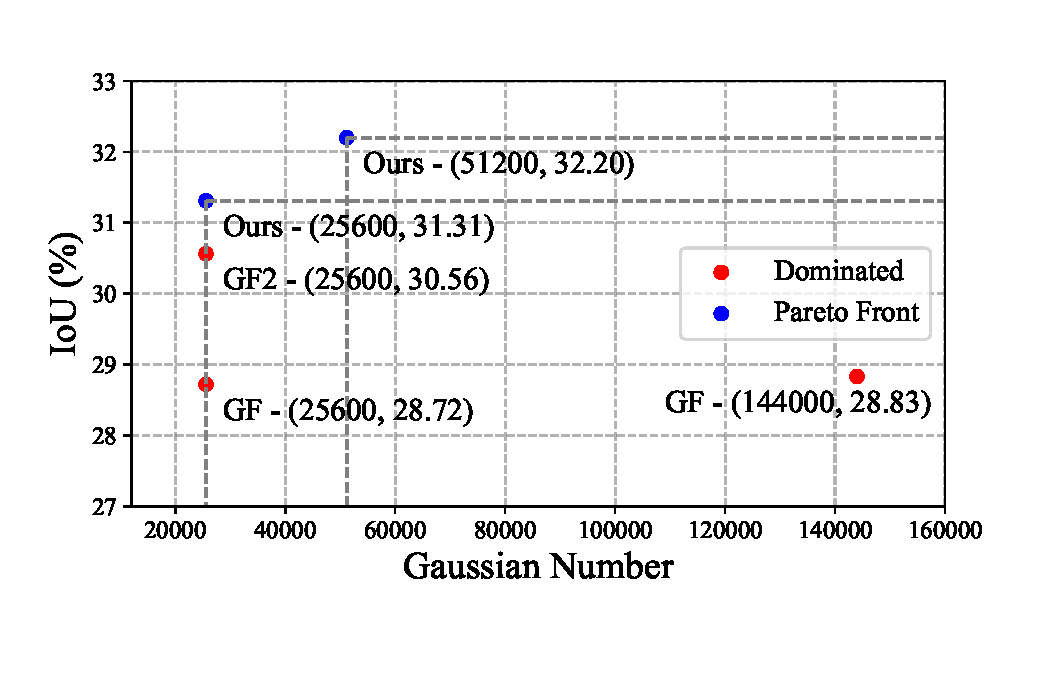
\includegraphics[width= 0.98\linewidth,trim={24 45 33 35},clip]{figures/pareto_plot.pdf}
    \caption{The Pareto front results of various Gaussian numbers and accuracy. Ours (blue) dominates others (red).}
    \label{fig:pareto}
\end{figure}

Finally, we manually selected 227 samples as an occlusion dataset and conducted an ablation study on the occlusion dataset to further validate the performance of Gaussian feature aggregation in our RoGaussianOCC for occlusion scenes.
% 为进一步验证GFA Module在遮挡场景下的的鲁棒性，我们人工标注了包含200+样本的遮挡数据集，并在该数据集上对模块进行消融实验。
The results in \autoref{tab:occlusiondataset} show that the historical Gaussian fusion leads to a $9.99\%$ IoU and $14.2\%$ mIoU improvements.
The Gaussian feature aggregation contributes to improvements of $1.17\%$ and $2.23\%$ in IoU and mIoU, respectively.



\begin{table*}[!ht] \centering \footnotesize
    \caption{The comparison between our RoGaussianOCC and the state-of-the-art vision-based occupancy predictions on nuScenes datasets, where the performance of GaussianFormer is the baseline. Memory Data is reported from GaussianFormer-2\cite{gaussianformer2}. $\dagger$ is referenced in OctreeOCC \cite{lu2024octreeoccefficientmultigranularityoccupancy}. $\ddagger$ and * represent the Gaussian numbers of 144000 and 25600, respectively.}
    % The data in bold and with a gray background, as well as in bold and italicized, represent the top three ideal scores.
    \label{tab:total}
    \setlength{\tabcolsep}{0.8pt}  
    \renewcommand\arraystretch{1.0}
    % \resizebox{\textwidth}{!}{%调整宽度
    \begin{tabular}{l | c | c c | c c c c c c c c c c c c c c c}   \toprule
        Method & \rotatebox{90}{\makecell{Memory\\(MB)}} &  \makecell{IoU(\%)} & \makecell{mIoU(\%)}
        & \rotatebox{90}{barrier}
        & \rotatebox{90}{bicycle}
        & \rotatebox{90}{bus}
        & \rotatebox{90}{car}
        % & \rotatebox{90}{const. veh.}
        & \rotatebox{90}{motor.}
        & \rotatebox{90}{pedes.}
        & \rotatebox{90}{\makecell[l]{traffic \\ cone}}
        & \rotatebox{90}{trailer}
        & \rotatebox{90}{truck}
        & \rotatebox{90}{\makecell[l]{drive. \\ suf.}}
        & \rotatebox{90}{other flat}
        & \rotatebox{90}{sidewalk}
        & \rotatebox{90}{terrain}
        & \rotatebox{90}{manmade}
        & \rotatebox{90}{vegetation}  \\  \midrule

MonoScene~\cite{monoscene}& - & 23.96 & 7.31 & 4.03 & 0.35 & 8.00 & 8.04 & 0.28 & 1.16 & 0.67 & 4.01 & 4.35 & 27.72 & 5.20 & 15.13 & 11.29 & 9.03 & 14.86 \\
Atlas~\cite{atlas}& - & 28.66 & 15.00 & 10.64 & 5.68 & 19.66 & 24.94 & 8.84 & 6.47 & 3.28 & 10.42 & 16.21 & 34.86 & 15.46 & 21.89 & 20.95 & 11.21 & 20.54 \\
BEVFormer~\cite{bevformer}&  25100 & 30.50 & 16.75 & 14.22 & 6.58 & 23.46 & 28.28 & 10.77 & 6.64 & 4.05 & 11.20 & 17.78 & 37.28 & 18.00 & 22.88 & 22.17 & 13.80 & 22.21 \\
TPVFormer~\cite{tpvformer}&  29000 & 30.86 & 17.10 & 15.96 & 5.31 & 23.86 & 27.32 & 8.74 & 7.09 & 5.20 & 10.97 & 19.22 & 38.87 & 21.25 & 24.26 & 23.15 & 11.73 & 20.81 \\
OccFormer~\cite{zhang2023occformer}& $>$22400$\dagger$ & 31.39 & 19.03 & 18.65 & 10.41 & 23.92 & 30.29 & 14.19 & \textbf{13.59} & \textbf{10.13} & 12.49 & 20.77 & 38.78 & 19.79 & 24.19 & 22.21 & 13.48 & 21.35 \\
\rowcolor{gray!30} GaussianFormer$\ddagger$~\cite{huang2024gaussianformer} & 6229 & 29.83 & 19.10 & 19.52 & 11.26 & 26.11 & 29.78 & 13.83 & 12.58 & 8.67 & 12.74 & 21.57 & 39.63 & 23.28 & 24.46 & 22.99 & 9.59 & 19.12 \\
GaussianFormer-2*\cite{gaussianformer2}& 3063 & 30.56 & 20.02 & 20.15 & 12.99 & \textbf{27.61} & 30.23 & 15.31 & 12.64 & 9.63 & 13.31 & \textbf{22.26} & 39.68 & 23.47 & 25.62 & 23.20 & 12.25 & 20.73 \\ \midrule
\rowcolor{gray!30}
\textbf{Ours(25600)}& 4680 & 31.31 (4.96\%$\uparrow$) & 20.22 (5.86\%$\uparrow$) & 19.38 & 13.05 & 27.01 & 30.16 & 15.52 & 13.11 & 9.29 & \textbf{13.83} & 21.95 & 39.92 & \textbf{23.88} & 25.72 & 23.63 & 13.33 & 22.71 \\
\rowcolor{gray!50}
\textbf{Ours(51200)}& 5508 & \textbf{32.20(7.95\%$\uparrow$)} & \textbf{20.65(8.12\%$\uparrow$)} & \textbf{20.28} & \textbf{13.05} & 27.30 & \textbf{30.48} & \textbf{16.21} & 13.47 & 9.71 & 13.42 & 22.25 & \textbf{40.39} & 23.81 & \textbf{26.26} & \textbf{24.16} & \textbf{14.85} & \textbf{23.80} \\ \bottomrule
\end{tabular}
\end{table*}


%%%%%%%
\begin{table}[!ht] \centering \footnotesize
\caption{The results of RoGaussianOCC on the occlusion dataset with common occluded objects.}
\label{tab:occlusiondataset}
\setlength{\tabcolsep}{2pt} \renewcommand\arraystretch{1.0}
\resizebox{\linewidth}{!}{
\begin{tabular}{l|c c |c c c c c c} \toprule
Method (*+PS) & IoU(\%) & mIoU(\%) & Barrier & Car & Ped. & Tra. \\ \midrule
Ours (HGF) & 27.04 (9.99\%$\downarrow$) &  18.86 (14.2\%$\downarrow$) & 15.96 & 26.48 & 10.83 & 8.90 \\
Ours (GA) & 29.69 (1.17\%$\downarrow$) &  21.49 (2.23\%$\downarrow$) & 19.63 & 30.29 & 12.81 & 12.58 \\ 
Ours (HGF+GA) & \textbf{30.04} & \textbf{21.98} & \textbf{21.55} & \textbf{30.52} & \textbf{13.36} & \textbf{13.08}    \\ \bottomrule
\end{tabular}}
\end{table}
%%%%%%%

%%%%%%%%%%%%%%%%%%%%%%%%%%
\subsection{Occupancy Prediction}
%%%%%%%%%%%%%%%%%%%%%%%%%%

%1. Total_vis
\begin{figure*}[!b] \centering \small
\includegraphics[width=0.98\textwidth,page=5,trim={129 67 143 75},clip]{figures/figures.pdf}
\caption{Visualization of Gaussian representation and occupancy prediction of our RoGaussianOCC on the nuScenes dataset.
}
\label{fig:visualization}
\end{figure*}


% In \autoref{tab:total}, 
We compare RoGaussianOCC to the state-of-the-art vision-based occupancy predictions on the nuScenes dataset, as shown in \autoref{tab:total}, where the performance of GaussianFormer is selected as the baseline.
% , using occupancy network annotations provided by SurroundOcc \cite{wei2023surroundocc}. 
% 在\autoref{tab:total}中，我们在nuScenes数据集，基于SurroundOcc\cite{wei2023surroundocc}提供的占用网络标注，将RoGaussianOCC与其他SOTA的纯视觉OCC预测模型进行对比。
% Compared to methods based on planar representations \cite{bevformer, tpvformer}, 
The results show that our RoGaussianOCC significantly outperforms the well-known BEV-based methods, such as BEVFormer \cite{bevformer} and TPVFormer \cite{tpvformer}.
For example, our RoGaussianOCC ({\small$\mathcal{N}$=25600}) performs an improvement of 1.46\% IoU and 18.25\% mIoU compared to TPVFormer.
% 与平面表示的方法\cite{bevformer,tpvformer}相比，我们的模型全面超越了先前工作，以0.69\%,0.2\%的几何IoU和语义mIoU相对提升取得了SOTA 
% 这里是51200相对于TPVFormer吗？
% Compared to methods based on dense grid representations,
Furthermore, RoGaussianOCC performs with an accuracy of approximately the same or higher than that of occupancy prediction methods with dense grid representation. 
For example, RoGaussianOCC ({\small$\mathcal{N}$=25600}) and RoGaussianOCC ({\small$\mathcal{N}$=51200}) perform
6.25\% and 8.51\% mIoU improvements, respectively, compared to the dense grid representation method OccFormer \cite{zhang2023occformer}.

Finally, our RoGaussianOCC with the same Gaussian numbers (25600) performs higher accuracy than the existing Gaussian occupancy predictions, such as GaussianFormer \cite{huang2024gaussianformer} and GaussianFormer-2 \cite{gaussianformer2}.
Specifically, our RoGaussianOCC with a Gaussian number of 25600 outperforms GaussianFormer with an improvement of 4.96\% IoU and 5.86\% mIoU, and outperforms GaussianFormer-2 with an improvement of 2.45\% IoU and 1.00\% mIoU.
For a larger Gaussian number of 51200, our RoGaussianOCC achieves an improvement of 7.95\% in IoU and 8.12\% in mIoU compared to GaussianFormer, respectively.


%%%%%%%%%%%%%%%%%%%%%%
\subsection{Visualization Results}
%%%%%%%%%%%%%%%%%%%%%%


%3. 遮挡数据集 GFA_Ablation_vis
\begin{figure*}[!b]\centering
\includegraphics[width=0.99\textwidth,page=7,trim={185 95 215 99},clip]{figures/figures.pdf}
\caption{
Visualization of a Gaussian distribution. 
Our RoGaussianOCC with historical Gaussian fusion reduces redundant Gaussian representations in empty regions and increases the Gaussian density in regions of interest (e.g., roadways). 
The percentage is the ratio of the accurate Gaussians to all Gaussians. 
The red and light blue dots represent the accurate Gaussian whose mean value is within the voxel and out of the voxel, respectively.
}
\label{fig:HGF_ablation}
\end{figure*}

%2. HGF_ablation_vis
\begin{figure*}[!ht] \centering
\includegraphics[width=0.99\linewidth,page=6,trim={123 52 120 69},clip]{figures/figures.pdf}
\caption{Visualization of occupancy prediction with Gaussian feature aggregation. TP: true positives, FN: false negatives.
}
\label{fig:GFA_ablation}
\end{figure*}


We conduct a qualitative analysis of the occupancy prediction results of RoGaussianOCC.
First, we present the visualization results of occupancy prediction of three representative scenes from nuScenes, as shown in \autoref{fig:visualization}.
% {请添加细节，图中表示了什么信息，具体怎么了}
% 第一组可视化是遮挡场景的典型案例，在车辆的后视角中，有一辆车被黑色小汽车遮挡(绿色框内）。
% GaussianFormer作为以单帧视觉输入的模型，无法利用时序信息，对之前视角出现过的汽车进行进行预测。
% 而我们的模型在使用了Gaussian Fusion和Aggregation策略后，可以针对连续的时序场景进行建模，成功预测被遮挡的车辆。
% GauianFormer由于依赖于单帧推理，容易造成空间信息在时序上的不一致，如图中的distant car，GaussiaFormer在前序帧可以成功预测，但在某个特定的视角，无法成功预测该车辆。我们的模型通过时序信息提取建模实现了在刁钻场景下的预测。此外，对于存在重叠的case，gaussianformer中的语义混淆体现了对语义不连续新。在空间连续性外，我们模型同时也提高了语义连续性，成功预测除了后方的巴士与前方的汽车。
% \todo[inline]{please describe the specific results in the visualization in Chinese. Done.}
The visual results show that our RoGaussianOCC accurately predicts the occupancy and semantics of small objects and occluded objects.
Specifically, the truck in the front view of the first scene (first row in \autoref{fig:visualization}) is partially occluded by a car, which is correctly predicted by our RoGaussianOCC but incorrectly by GaussianFormer, as GaussianFormer with single-frame input predicts occupancy without temporal information.
A distant car in the second scene (second row in \autoref{fig:visualization}) is ignored by GaussianFormer since the distant car is viewed as a small object, while it is predicted by our RoGaussianOCC.
The third scene (third row) demonstrates that our RoGaussianOCC accurately predicts occupancy in the dark scene, whereas GaussianFormer predicts occupancy incorrectly.
Our GaussianFormer predicts the occupancy for the scene of a car overlapped with a bus (fourth row), which GaussianFormer predicts incorrectly. 
% in the current frame through temporal fusion.
% 我们对RoGaussianOCC的预测结果做了定性分析。RoGaussianOCC在时序信息与时空融合下，可以预测更加全面的场景，同时能够概括场景中物体的精细轮廓。

Furthermore, we observe the visual results of the Gaussian distribution caused by historical Gaussian fusion, as shown in \autoref{fig:HGF_ablation} where the red dots represent the accurate Gaussian whose mean value is in the voxel.
% {请添加细节，图中表示了什么信息，具体怎么了}
% \todo[inline]{please describe the specific results in the visualization in Chinese. Done}
% 在这个图中，在消融实验中，我们可视化了historical Gaussian Fussion对于提升高斯efficiency的实验结果，红色点代表均值在体素内的的高斯，而下方的数字代表的是Pers评分，既准确高斯的占比。在图中的三个case，得分从低到高分别为GaussianFormer，我们消融掉HGF模块后的模型，以及我们的模型。其次，有效高斯（红色点）也更集中在道路中心区域。这些现象说明了，我们的HGF可以提高约1%的高斯效率，而其他模块（GA,PS）对比GaussianFormer也有约0.5%的高斯效率提升。
The percentage is the ratio of the accurate Gaussians to all Gaussians.
\autoref{fig:HGF_ablation} shows three various scenes with low to high accurate Gaussians. 
The visual results show that Gaussians in our RoGaussianOCC are concentrated in the regions of interest that require intensive Gaussian representations, which reduces Gaussian redundancy in empty regions and has higher {\small $\mathcal{P}_p$} scores than GaussianFormer.
For example, the Gaussians are concentrated on the road and the objects on both sides that are key occupancies to autonomous driving.
% 我们通过对比在不同场景下高斯的最终位置，对HGF模块了开展了消融实验。
% 在HGF模块的帮助下，能够将更多的高斯集中在需要高密度的复杂区域中，并减少低密度区域高斯冗余的情况，这有利于表示复杂场景的细节。

Finally, we present the visual results of Gaussian feature aggregation of three representative scenes in \autoref{fig:GFA_ablation}.
% {请添加细节，图中表示了什么信息，具体怎么了}
% \todo[inline]{please describe the specific results in the visualization in Chinese.Done}
% 我们可视化了GA模块的消融实验对比结果。
% 在Scene1的场景中，自车的后方，有两辆车（如gt所示），而第二辆车被第一辆车所遮挡（绿色框内），我们在消融掉GFA模块后，模型无法正确预测正后方被遮挡的车辆，而我们采用了GFA模块的模型，成功对后方的车辆进行了预测。
The visual results show that our RoGaussianOCC with Gaussian feature aggregation performs accurate occupancy predictions for occluded objects. 
% \vspace{1cm}
% 对比有无Gaussian feature aggregation模块在实际场景中的可视化结果，可以发现使用GFA模块后，预测的范围更大，且更准确。
In the first scene (first row), the targeted car behind the ego-vehicle is partially occluded, which is correctly predicted by our RoGaussianOCC with GFA and incorrectly predicted without GFA, respectively.   
% 在Scene2的场景中，自车位于视野狭窄的车道，并且前方有多辆车，且存在视野遮挡（gt中绿框所示），这是自动驾驶中极具挑战性的场景。
In the second scene, our RoGaussianOCC with GFA accurately predicts occupancy for the challenging scenario of multiple vehicles on a narrow road.
% This is an extremely challenging scenario in autonomous driving.
% 根据消融实验，我们的模型确实可以对车道左前方被遮挡的车进行准确的几何与语义预测，验证了GFA模块对遮挡场景的有有效性。
In the third scene, our RoGaussianOCC with GFA module correctly predicts the occupancy of a truck at the crossroads. 


%%%%%%%%%%%%%%%%%%%%%%%%%%%%%%%%
\section{Discussion}
\label{sec:discussion}
%%%%%%%%%%%%%%%%%%%%%%%%%%%%%%%%

Although our RoGaussianOCC shows remarkable performance in occupancy predictions, there are still many interesting issues that need to be further investigated.
% 验过程中，我们还发现了一些值得讨论的现象。
First, we observed that Gaussian occupancy prediction methods based on deformable attention, including our RoGaussianOCC, still require further improvement for small objects.
This issue is generally caused by two reasons: 1) small objects are assigned fewer Gaussians, resulting in weak feature representation; 2) small objects are often partly occluded and thus are hardly predicted.
% 我们注意到，包括RoGaussianOCC在内的，基于deformable attention的一系列高斯occ方法相较于传统occ方法，都在体积较小的对象（如行人、traffic cone）表现不佳，原因可能，1.体积小的对象分配到的高斯数目少，导致对细节的表示能力差；2.小物体特征点少且容易被遮挡，模型难识别
% \subsection{Limitations}
% 我们的模型存在以下潜在问题，这可能会导致模型表现不佳。
% 我们的GFA仅仅是在输入流中直接采取前序关键帧作为时序融合信息，并未根据车辆运行的实际情况选取历史信息足够充分的前序帧。
% 在后续的工作中，我们考虑加入对历史帧信息的选择纳入研究范围。
Second, the Gaussian feature aggregation in our RoGaussianOCC considers the previous keyframes as a form of temporal fusion.
However, frames with efficient historical information can be selected based on the vehicle's historical path.
In the future, we will select historical keyframes by considering the vehicle's historical path.
% GFA模块中车辆速度缓慢或停止时，前序帧与当前帧的视角差异不大，4D的特征融合可能会退化成3D特征融合:
% 我们的GFA中仅仅是在输入流中直接采取前序关键帧作为时序融合信息，并未根据车辆运行的实际情况选取历史信息足够充分的前序帧。例如：车辆在停止或者缓慢行驶过程中，前序帧与当前帧的视角差距不够大。在后续的工作中，我们考虑加入对历史帧信息的选择纳入研究范围。
Third, the ego-motion alignment in the historical Gaussian fusion of our RoGaussianOCC only considers the motion of the ego vehicle, ignoring the motion of other moving objects.
Considering that all motion objects may improve Gaussian occupancy predictions.
% Our model has inaccurate predictions in some scenes. We speculate that this may be because RoGaussianOCC does not consider the relative motion of objects, resulting in poor fitting results.
% EGA中的ego-motion alignment仅考虑了车辆自身的运动而忽视了其他物体运动，可能会导致预测不准确。
% 我们的模型在部分场景存在预测不准确的情况，我们推测可能是因为RoGaussianOCC没有考虑物体相对运动的过程，导致拟合结果不佳。


% \todo[inline]{上面三个讨论是关于方法论， 我们还可以添加关于实验的讨论， 包括实验设置， 实验结论有什么缺点， 特殊， 异常。 例如，我们的消融实验有什么局限（真的重大bug反而可以不提，要不然找拒），消融实验的结论，有什么异常，以及异常的hyperthesis是什么， 对比实验中，有什么异常以及有意思的间接结论。}


%1） 我提出的方法（三个模块组成的RoGaussianOCC）中存在的潜在不足以及可能的提升方案。

% 1.  GA中的ego-motion alignment仅考虑了车辆自身的运动而忽视了其他物体运动，可能会导致预测不准确。
% 我们的模型在部分场景存在预测不准确的情况，我们推测可能是因为RoGaussianOCC没有考虑物体相对运动的过程，导致拟合结果不佳。
In the GFA module, the ego-motion alignment only considers the movement of the ego-vehicle but ignores the movement of other traffic objects, which may lead to underfitting results.
The movement of other traffic objects may contribute to improving occupancy prediction.
% Our model has inaccurate predictions in some scenes. We speculate that this may be because RoGaussianOCC does not consider the relative motion of objects, resulting in poor fitting results.
% 2. GFA模块中，我们采用固定时序采样帧率，车辆速度缓慢或停止时，前序帧与当前帧的视角差异不大，4D的特征融合可能会退化成3D特征融合。 
% 因此，我们收到OpenFly启发，\cite{gao2025openflyversatiletoolchainlargescale},利用自车ego motion信息建模车辆行驶的时序信息，在高速/转弯等用视角改变大的动作时进行关键帧采样，更好的融合时序信息。
Additionally, we employ a fixed temporal sampling frame rate, which results in inefficient Gaussian feature aggregation when the vehicle is moving slowly or stopped.
% since the temporal perspective difference between the previous frame and the current frame is not large, and the 4D feature fusion may degenerate into 3D feature fusion.
To address this issue, we will utilize the ego-vehicle motion information to model temporal information for key frame sampling, thereby adapting to low- or high-speed driving scenes \cite{gao2025openfly}.
% for  and other actions with large perspective changes, and better integrate the timing information.
% 3. 我们引入了Perspective supervision 用来直接监督backbone，但当前的loss中的评估指标不够全面。
% 当前，gaussianOCC的技术路径，都是通过将高斯splatting为OCC，并且用selfocc-nuscenes 提供的OCC标注作为groudtruth进行训练。
% 该监督信号直接作用于溅射后的OCC，不能对高斯进行直接的指导，缺乏对高斯准确度的直接监督信号。
% 因此，我们可以考虑引入GaussianFormer2 中关于高斯L1 Distance, overlay 重叠率的指标，用于总和评估模型表现。此外，还可以考虑利用现有OCC标注与Nuscenes使用3D重建的方法，生成一组3D Gaussian gt，用于直接训练semantic高斯。
Although we introduced perspective supervision to train the backbone, it is directly applied to occupancy prediction and cannot provide supervision for Gaussians.
In the future, we will introduce the Gaussian L1 distance and the overlay to comprehensively evaluate the performance.
Additionally, we will utilize the occupancy annotation of nuScenes to generate ground truth for Gaussian training.


% 2）我们的实验设置中存在哪些不足，以及可以改进的方向
%例如数据集设置是否不合理，消融实验是否存在不完美的地方。
% 目前，我们使用Perspective supervision head 对backbone进行监督，我们可以多尝试同的监督头，进行消融实验。
% 此外，我们没有进行对历史帧数量选择的消融实验，后续也可以在加入keyframe selector后进行进一步消融实验。

%3） 我们的实验结果中存在哪些异常，而当前的实验结果没有直接说明异常的原因。对于这些问题，可以给出自己的合理分析和猜测。以及是否重要，对我们的整体结果是否有影响等等分析。

Although our RoGaussianOCC outperforms other methods, OccFormer outperforms our RoGaussianOCC in terms of pedestrian and traffic cone, as shown in \autoref{tab:total}.
% 1. 在我们的实验中，我们对pedestrian, traffic cone 等物体的感知能力并不是SOTA。
% 6.6 更新
% 我们注意到，包括RoGaussianOCC在内的，基于deformable attention的一系列高斯occ方法（gaussianformer）相较于传统occ(occ former)方法，都在体积较小的对象（如行人、traffic cone）表现不佳。
We noticed that deformable attention-based Gaussian occupancy prediction methods (RoGaussianOCC) generally perform weaker on small objects (such as pedestrians and traffic cones) than traditional occupancy prediction methods, such as OccFormer.
% 体积小的对象分配到的高斯数量少，在小范围区域内需要更多高斯叠加，才可以在gaussian to occ模块中，拥有更高的置信度，从而转化为occupancy。
Small objects are assigned a few Gaussians that are hardly to be predicted as occupancy.
%相反，以voxel作为representation的传统occ方法，可以直接对小物体的区域进行decode。
In contrast, traditional occupancy prediction methods that use voxels as the representation can accurately decode small objects and predict them as occupied.
In the future, we will incorporate confidence into Gaussians to enhance the occupancy prediction of small objects.  


%%%%%%%%%%%%%%%%%%%%%%%%%%%%%%%%
\section{Conclusions}
\label{sec:conclusions}
%%%%%%%%%%%%%%%%%%%%%%%%%%%%%%%%

In this work, we proposed a novel Gaussian occupancy prediction, RoGaussianOCC, to improve the efficiency and robustness by considering three key modules: 1) historical Gaussian fusion, 2) Gaussian feature aggregation, and 3) perspective supervision.
We conducted an ablation study to validate the contributions of the three novel modules to the improvement of occupancy prediction and compared RoGaussianOCC to state-of-the-art occupancy predictions (e.g., Gaussianformer, Gaussianformer-2) on the well-known nuScenes dataset.
The results demonstrate that our RoGaussianOCC outperforms existing Gaussian occupancy predictions (e.g., GaussianFormer and GaussianFormer-2) in terms of accuracy and robustness for autonomous driving applications.
The efficiency and robustness of occupancy prediction significantly provide the cornerstone for path planning and decision-making of autonomous driving. 
However, our work focused on the perception stage (occupancy prediction), a crucial step in autonomous driving, without validating the performance improvements it brings to the end-to-end autonomous driving system.
In the future, we will apply the proposed RoGaussianOCC to validate its contribution to the autonomous driving system and improve the performance of end-to-end autonomous driving.

% \newpage
% \vspace{-3pt}
\bibliographystyle{IEEEtran}
\bibliography{references}

% \vspace{-18mm}
\begin{IEEEbiography}
    [{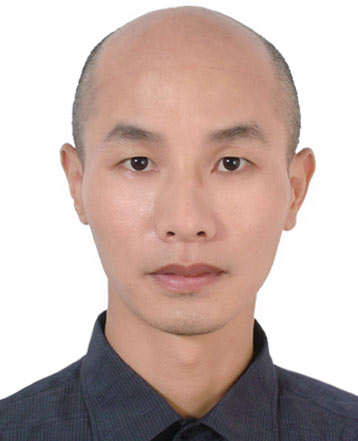
\includegraphics[width=1in,height=1.25in,trim={10 30 15 0}, clip, keepaspectratio]{figures/ID_GJ.jpg}}]
    {Gongjin Lan (Senior Member, IEEE)} is currently a Research Assistant Professor, Associate Researcher at the Department of Computer Science and Engineering, Southern University of Science and Technology, Shenzhen, China. 
    He received his PhD in Artificial Intelligence at VU Amsterdam in 2020, and published over 30 academic papers ($>$1000 citations, h-index=21) in top journals and conferences, including \textit{IEEE T-IV, IEEE THMS, IEEE TII, IEEE TLT, Swarm and Evolutionary Computation, Knowledge-Based Systems, Scientific Reports, PPSN}, and serves as a active reviewer for 15+ top journals/conferences (including \textit{Nature Communications, IEEE TEVC, IEEE THMS, IEEE TII, IEEE TMC, IEEE RA-L, Swarm and Evolutionary Computation, Scientific Reports, ICRA, IROS, GECCO, IJCNN}), the Guest Editor for a SCI-Q3 journal and the Session Chair at a top IEEE conference, the Secretary and Co-Founder of a IEEE ITSS Chapter. His research interests include autonomous driving, embodied AI, and interdisciplinary AI. 
\end{IEEEbiography}

\vspace{-38mm}
\begin{IEEEbiography}
    [{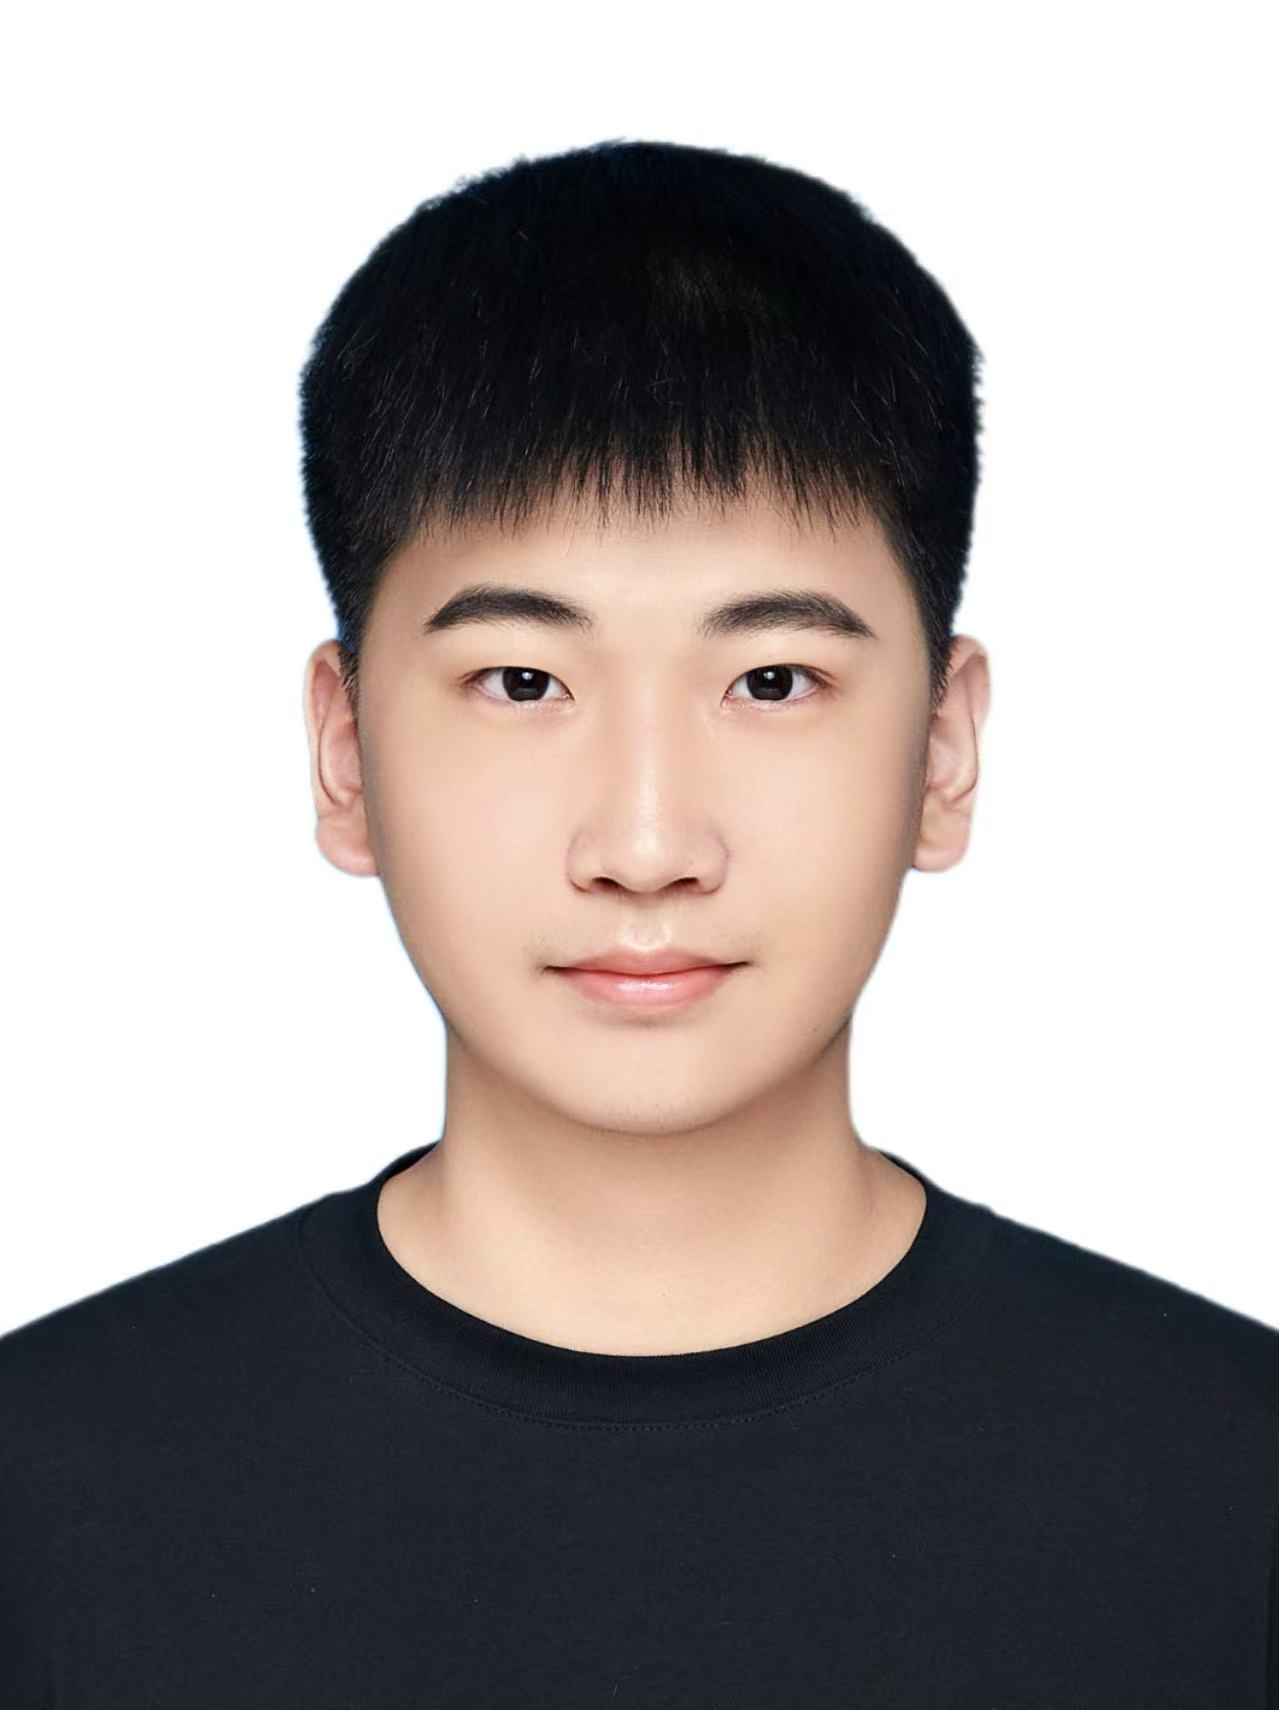
\includegraphics[width=1in,height=1.25in,trim={10 35 15 15}, clip, keepaspectratio]{figures/MJF_ID.jpg}}]
    {Jianfa Ma} is currently an undergraduate student at the Department of Computer Science and Engineering, Southern University of Science and Technology, Shenzhen, China. His research interests include the Occupancy Network, Embodied Intelligence, and Computer Vision.
\end{IEEEbiography}

\vspace{-38mm}
\begin{IEEEbiography}
    [{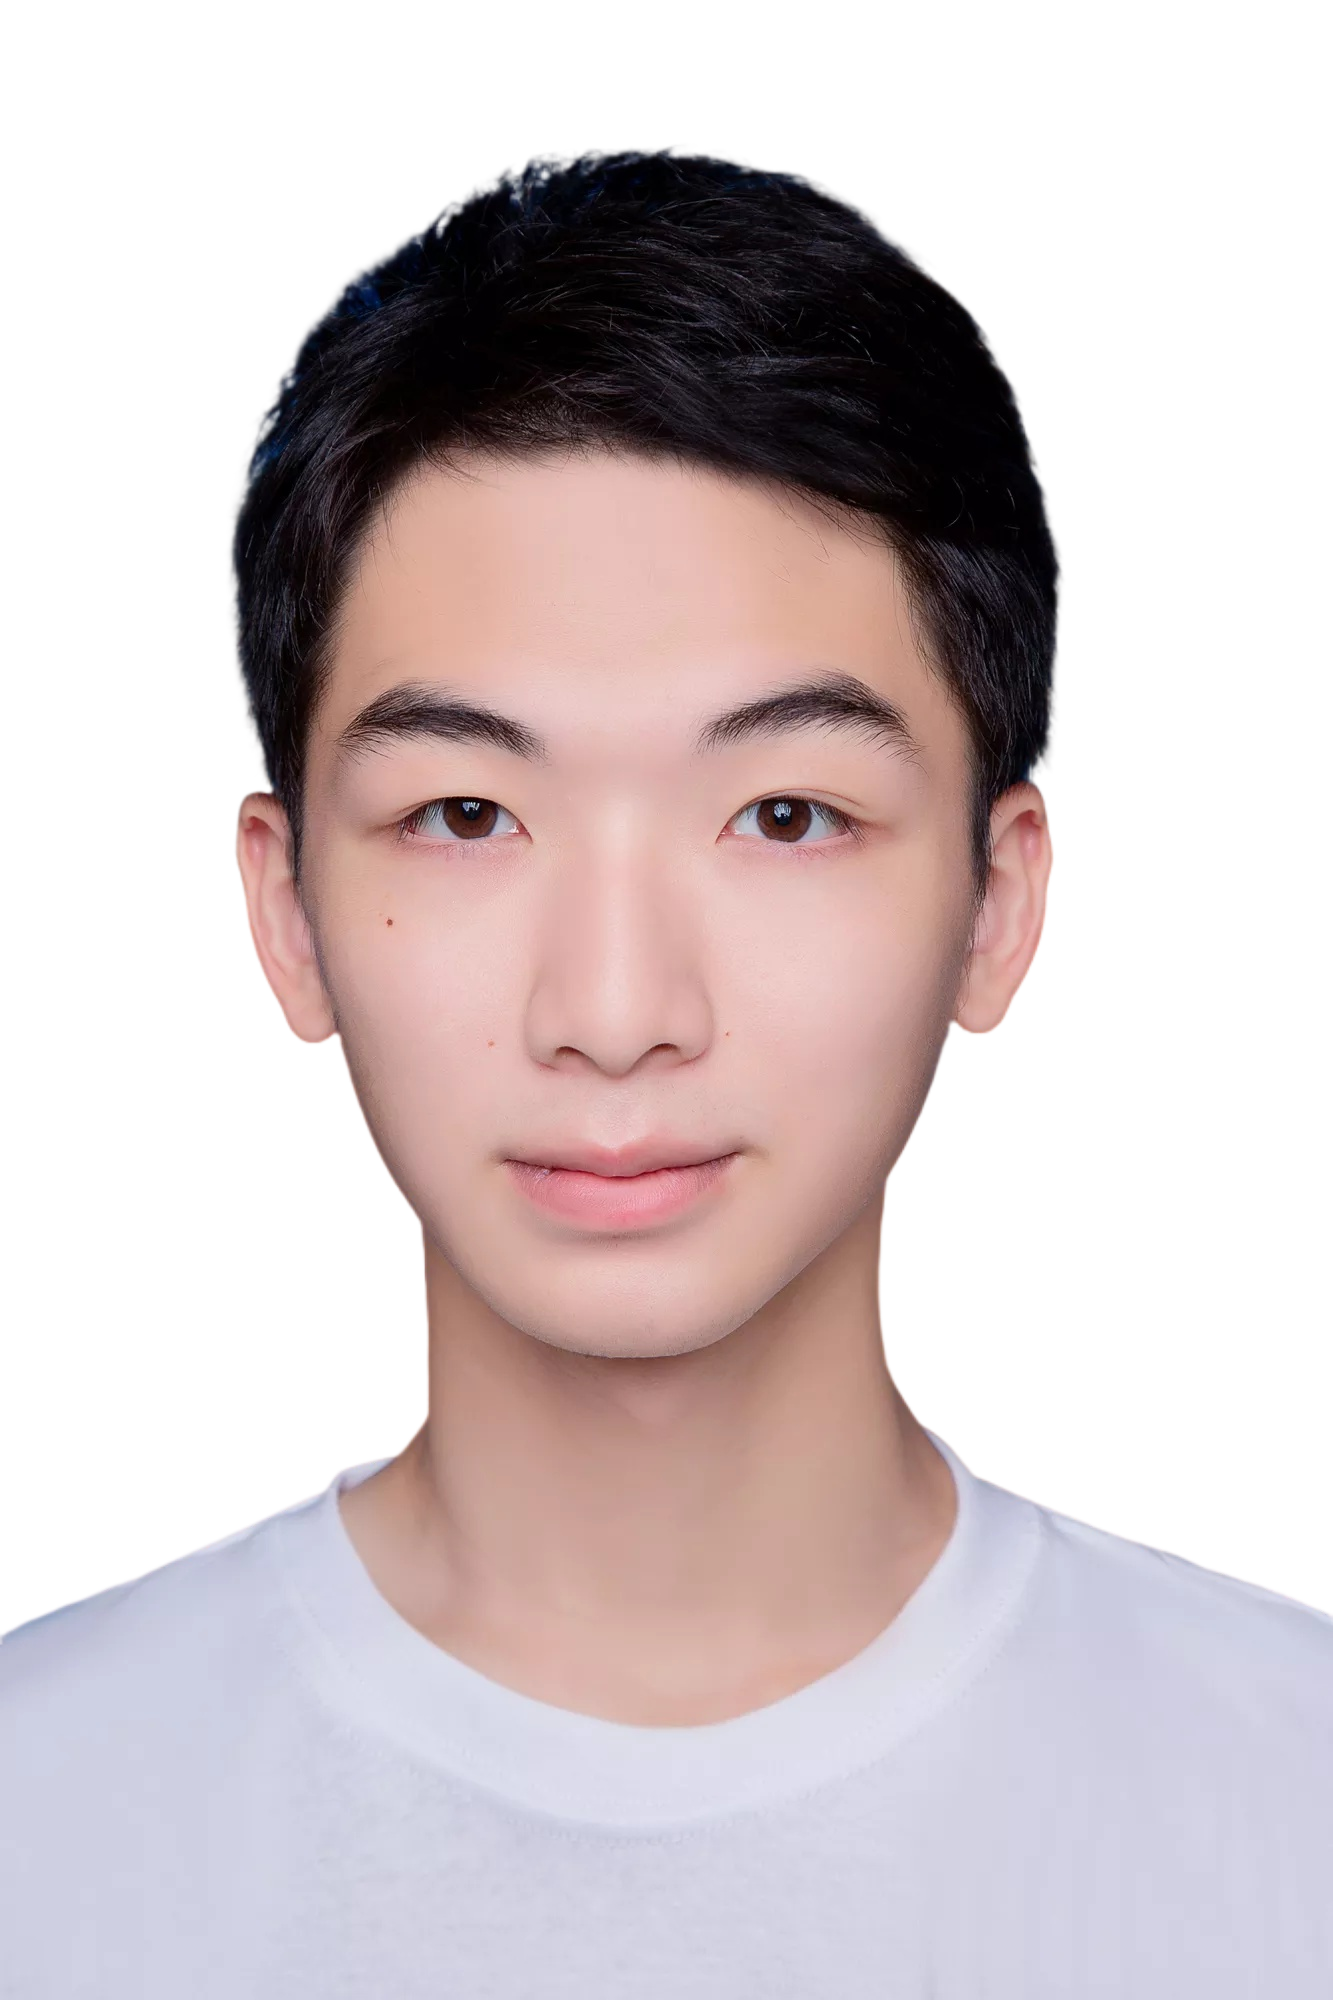
\includegraphics[width=1in,height=1.25in,trim={10 35 15 15}, clip, keepaspectratio]{figures/ZZY_ID.png}}]
    {Ziyue Zhao} is an undergraduate student majoring in Computer Science and Engineering, Southern University of Science and Technology, Shenzhen, China. 
    His research interests include autonomous driving, computer vision.
\end{IEEEbiography}

\newpage
% \vspace{-18mm}
\begin{IEEEbiography}
    [{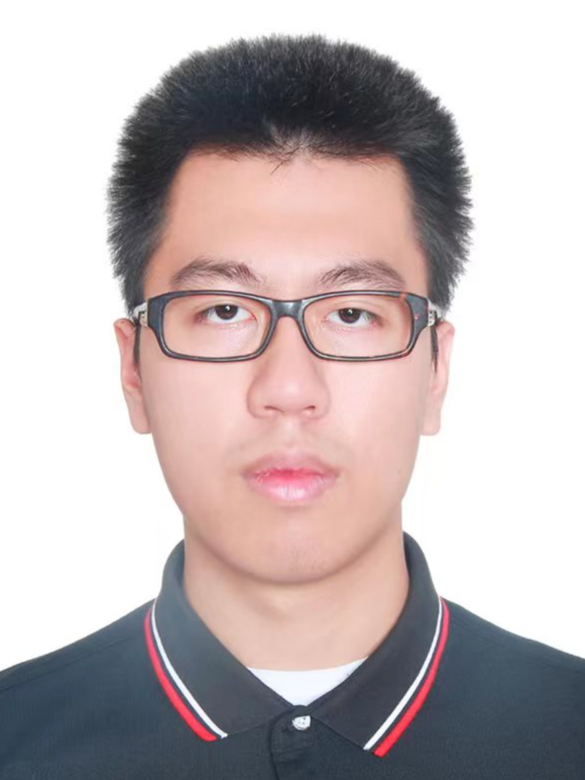
\includegraphics[width=1in,height=1.25in,trim={10 40 15 5}, clip, keepaspectratio]{figures/QN_Qi_ID.jpg}}]
    {Qining Qi} is an undergraduate student majoring in Computer Science and Engineering, Southern University of Science and Technology, Shenzhen, China. 
    His research interests include autonomous driving, computer vision, and information security.
\end{IEEEbiography}

\vspace{-38mm}
\begin{IEEEbiography}
    [{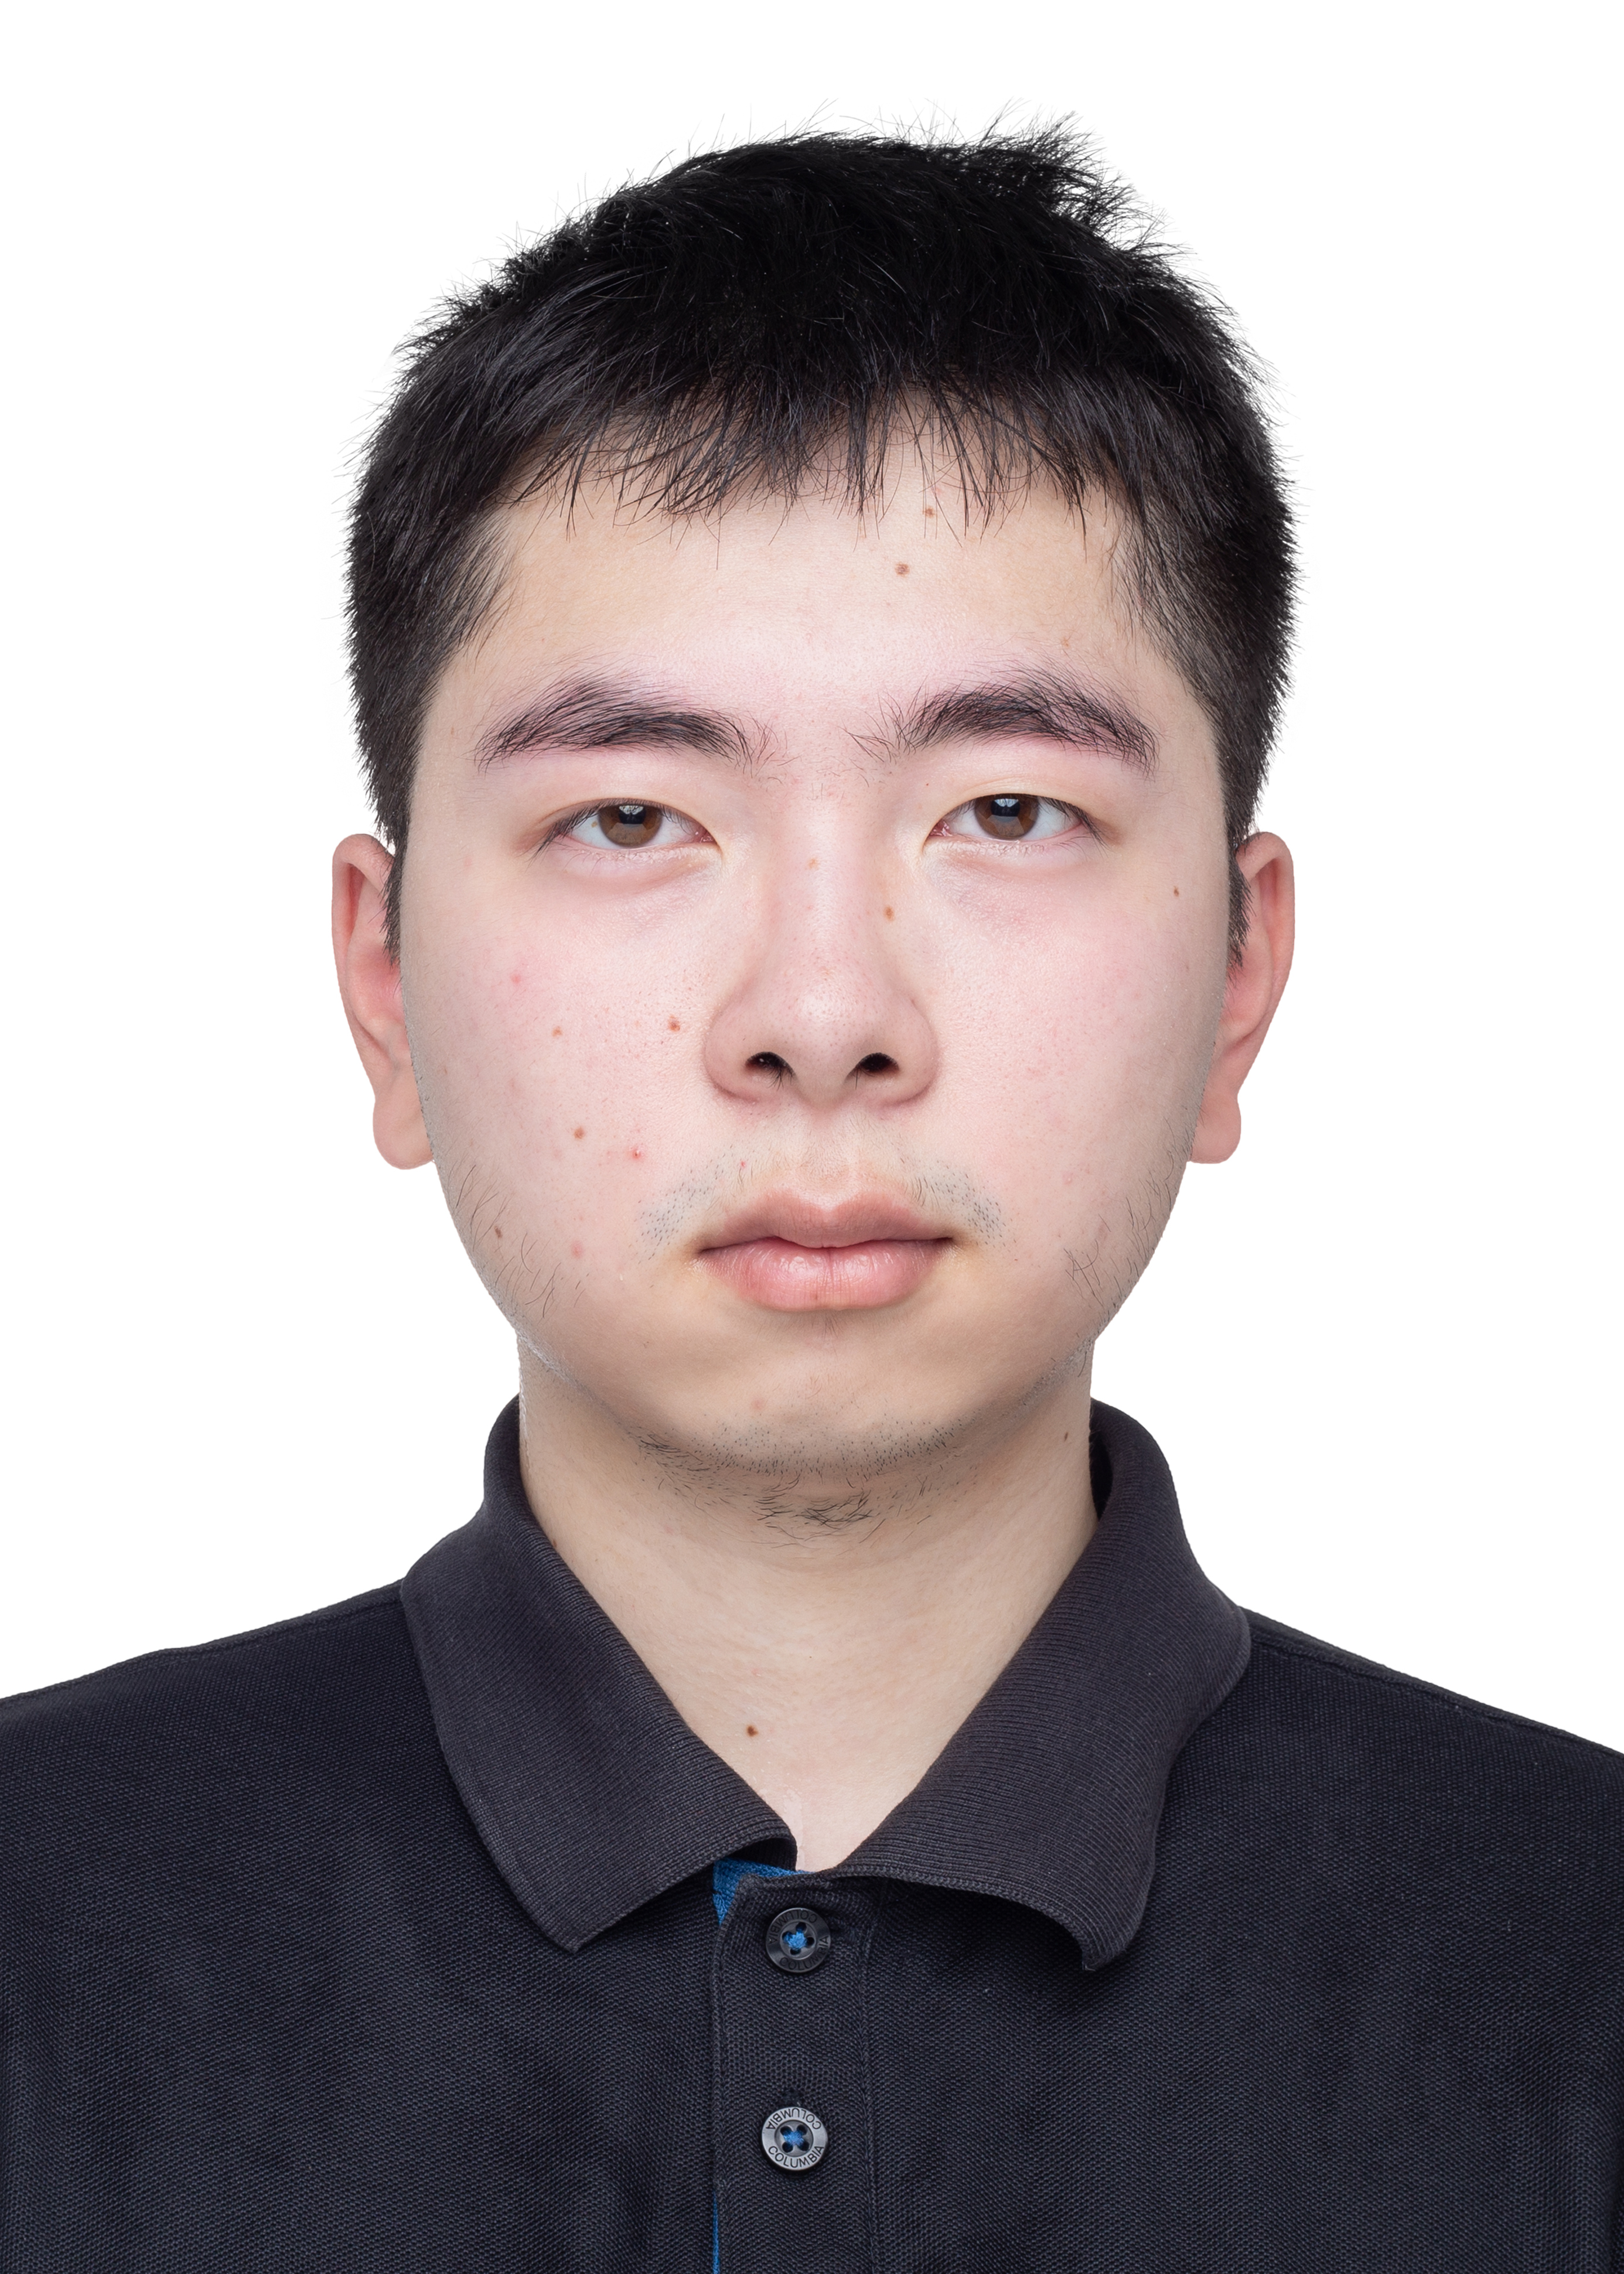
\includegraphics[width=1in,height=1.25in,trim={10 30 15 5}, clip, keepaspectratio]{figures/LYC_ID.jpg}}]
    {Yechong Liu} is a postgraduate student majoring in Computer Science and Engineering, Southern University of Science and Technology, Shenzhen, China. 
    His research interests include autonomous driving, computer vision, and robust learning.
\end{IEEEbiography}

\vspace{-38mm}
\begin{IEEEbiography}
    [{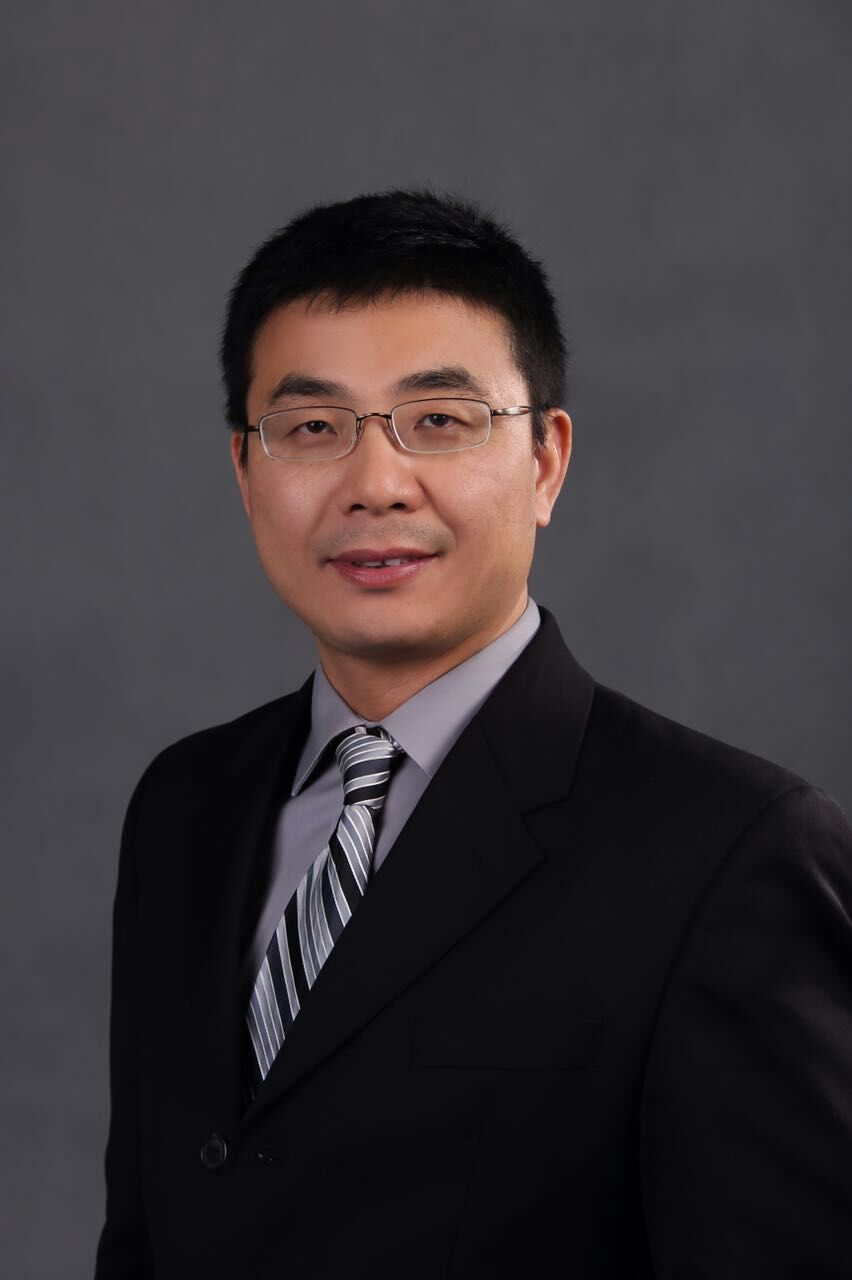
\includegraphics[width=1in,height=1.25in,trim={0 55 0 95},clip,keepaspectratio]{figures/Hao_ID.jpg}}]
    {Qi Hao (Senior Member, IEEE)} is currently a full Professor at the Southern University of Science and Technology, Shenzhen, China, the leader of the Intelligent Sensing and Unmanned Systems Lab, Executive Dean of the Research Institute of Trustworthy Autonomous Systems, Executive Director of SUSTech-Haylion Center for Intelligent Transportation, Deputy Director of Shenzhen Key Laboratory of Robotics and Computer Vision. 
    He received the B.E. and M.E. degrees from Shanghai Jiao Tong University, Shanghai, China, in 1994 and 1997, respectively, and the Ph.D. degree from Duke University, Durham, NC, USA, in 2006, all in electrical and computer engineering.
    % , was a Postdoctoral Fellow with the Center for Visualization and Virtual Environment, University of Kentucky, Lexington, KY, USA, focusing on 3D computer vision. 
    From 2007 to 2014, he was an Assistant Professor at the Department of Electrical and Computer Engineering, University of Alabama, Tuscaloosa, AL, USA. His current research interests include intelligent unmanned systems, machine learning, and smart sensors.
\end{IEEEbiography}

\end{document}